\documentclass[10pt,twocolumn,letterpaper]{article}

\usepackage{iccv}
\usepackage{times}
\usepackage{epsfig}
\usepackage{graphicx}
\usepackage{amsmath}
\usepackage{amssymb}

\usepackage[export]{adjustbox}
\usepackage{etoolbox}
\usepackage[normalem]{ulem}
\usepackage[symbol]{footmisc}

\usepackage{stmaryrd}
\usepackage{placeins}

\usepackage{adjustbox}
\usepackage{dcolumn}

\usepackage[square,sort,comma,numbers]{natbib}
\usepackage{multibib}
\newcites{appendix}{References}%


\usepackage[breaklinks=true,bookmarks=false]{hyperref}

\iccvfinalcopy %

\def\iccvPaperID{****} %
\def\httilde{\mbox{\tt\raisebox{-.5ex}{\symbol{126}}}}

\ificcvfinal\pagestyle{empty}\fi


\usepackage{times}
\usepackage{epsfig}
\usepackage{graphicx}
\usepackage{float}
\usepackage{wrapfig}
\usepackage{amsmath,amssymb,amsthm}
\usepackage{algorithm,algorithmicx,algpseudocode}
\usepackage{bm,xspace}
\usepackage{comment}
\usepackage{verbatim}
\usepackage{multirow}
\usepackage{balance}
\usepackage{url}
\usepackage{booktabs}
\usepackage{etoolbox,siunitx}
\usepackage{calc}
\usepackage{pifont,hologo}
\usepackage[usenames, dvipsnames]{color}
\usepackage{nicefrac}

\setlength\heavyrulewidth{0.10em}
\setlength\lightrulewidth{0.05em}
\setlength\cmidrulewidth{0.03em}
\newcommand{\ra}[1]{\renewcommand{\arraystretch}{#1}}

\usepackage[super]{nth}
\usepackage{nicefrac}
\sisetup{detect-weight=true,detect-inline-weight=math}
\sisetup{quotient-mode = fraction}
\sisetup{fraction-function = \nicefrac}
\robustify\bfseries


\def\aa{\mathbf{a}}
\def\bb{\mathbf{b}}
\def\cc{\mathbf{c}}
\def\dd{\mathbf{d}}
\def\ee{\mathbf{e}}
\def\ff{\mathbf{f}}
\def\gg{\mathbf{g}}
\def\hh{\mathbf{h}}
\def\ii{\mathbf{i}}
\def\jj{\mathbf{j}}
\def\kk{\mathbf{k}}
\def\ll{\mathbf{l}}
\def\mm{\mathbf{m}}
\def\nn{\mathbf{n}}
\def\oo{\mathbf{o}}
\def\pp{\mathbf{p}}
\def\qq{\mathbf{q}}
\def\rr{\mathbf{r}}
\def\sss{\mathbf{s}}
\def\ttt{\mathbf{t}}
\def\uu{\mathbf{u}}
\def\vv{\mathbf{v}}
\def\ww{\mathbf{w}}
\def\xx{\mathbf{x}}
\def\yy{\mathbf{y}}
\def\zz{\mathbf{z}}

\def\AA{\mathbf{A}}
\def\BB{\mathbf{B}}
\def\CC{\mathbf{C}}
\def\DD{\mathbf{D}}
\def\EE{\mathbf{E}}
\def\FF{\mathbf{F}}
\def\GG{\mathbf{G}}
\def\HH{\mathbf{H}}
\def\II{\mathbf{I}}
\def\JJ{\mathbf{J}}
\def\KK{\mathbf{K}}
\def\LL{\mathbf{L}}
\def\MM{\mathbf{M}}
\def\NN{\mathbf{N}}
\def\OO{\mathbf{O}}
\def\PP{\mathbf{P}}
\def\QQ{\mathbf{Q}}
\def\RR{\mathbf{R}}
\def\SS{\mathbf{S}}
\def\TT{\mathbf{T}}
\def\UU{\mathbf{U}}
\def\VV{\mathbf{V}}
\def\WW{\mathbf{W}}
\def\XX{\mathbf{X}}
\def\YY{\mathbf{Y}}
\def\ZZ{\mathbf{Z}}

\def\aA{\mathcal{A}}
\def\bB{\mathcal{B}}
\def\cC{\mathcal{C}}
\def\dD{\mathcal{D}}
\def\eE{\mathcal{E}}
\def\fF{\mathcal{F}}
\def\gG{\mathcal{G}}
\def\hH{\mathcal{H}}
\def\iI{\mathcal{I}}
\def\jJ{\mathcal{J}}
\def\kK{\mathcal{K}}
\def\lL{\mathcal{L}}
\def\mM{\mathcal{M}}
\def\nN{\mathcal{N}}
\def\oO{\mathcal{O}}
\def\pP{\mathcal{P}}
\def\qQ{\mathcal{Q}}
\def\rR{\mathcal{R}}
\def\sS{\mathcal{S}}
\def\tT{\mathcal{T}}
\def\uU{\mathcal{U}}
\def\vV{\mathcal{V}}
\def\wW{\mathcal{W}}
\def\xX{\mathcal{X}}
\def\yY{\mathcal{Y}}
\def\zZ{\mathcal{Z}}

\def\Ae{\mathbb{A}}
\def\Be{\mathbb{B}}
\def\Ce{\mathbb{C}}
\def\Le{\mathbb{L}}
\def\Ne{\mathbb{N}}
\def\Pe{\mathbb{P}}
\def\Qe{\mathbb{Q}}
\def\Re{\mathbb{R}}
\def\Se{\mathbb{S}}
\def\Te{\mathbb{T}}
\def\Xe{\mathbb{X}}
\def\Ye{\mathbb{Y}}
\def\Ze{\mathbb{Z}}

\def\btheta{{\bm\theta}}
\def\bTheta{{\bm\Theta}}
\def\bzeta{{\bm\zeta}}
\def\bmu{{\bm\mu}}
\def\bZero{\mathbf{0}}
\def\bOne{\mathbf{1}}

\DeclareMathOperator*{\argmax}{arg\,max}
\DeclareMathOperator*{\argmin}{arg\,min}
\DeclareMathOperator*{\minimize}{minimize}
\DeclareMathOperator*{\maximize}{minimize}

\DeclareMathOperator{\sign}{sign}
\DeclareMathOperator{\rank}{rank}
\DeclareMathOperator{\trace}{tr}
\DeclareMathOperator{\diag}{diag}
\DeclareMathOperator{\diam}{diam}

\def\eps{\varepsilon}
\def\vphi{\varphi}
\def\vsigma{\varsigma}

\def\trans{^{\top}}
\def\deg{^{\circ}}

\def\th{^{\textnormal{th}}}
\def\st{^{\textnormal{st}}}
\def\nd{^{\textnormal{nd}}}

\newcommand\ggreater{\mathbin{>\!\!\!>}}
\newcommand\llesser{\mathbin{<\!\!\!<}}

\newcommand{\YesV}{\ding{51}}%
\newcommand{\NoX}{\ding{55}}%

\DeclareMathSymbol{@}{\mathord}{letters}{"3B}

\newcommand\paren[1]{\left(#1\right)}
\newcommand\abs[1]{\left\lvert#1\right\rvert}
\newcommand\norm[1]{\left\lVert#1\right\rVert}
\newcommand\tuple[1]{\left\langle#1\right\rangle}
\newcommand\inner[2]{\langle #1, #2 \rangle}

\newcommand\timess{\mathbin{\!\times\!}}

\newcommand\nicebar[1]{\mkern 4mu\overline{\mkern-4mu#1}}

\newcommand\vladlen[1]{\textcolor{blue}{\bf Vladlen says: #1}}
\newcommand\rene[1]{\textcolor{Orange}{\bf Rene says: #1}}
\newcommand\alexey[1]{\textcolor{OliveGreen}{\bf Katrin says: #1}}
\newcommand\story[1]{\textcolor{red}{\bf TODO: #1}}

\newcommand\mypara[1]{\vspace{1mm}\noindent\textbf{#1}}

\def\rot#1{\rotatebox{90}{#1}}

\def\latex/{\LaTeX}
\def\bibtex/{\hologo{BibTeX}}


\def\Uline#1{#1\llap{\uline{\phantom{11.11}}}}

\begin{document}

\title{Vision Transformers for Dense Prediction\vspace{-0.5em}}

\author{Ren\'{e} Ranftl\\
  \and
  Alexey Bochkovskiy\\
  \\Intel Labs\\
  {\tt\small rene.ranftl@intel.com}\\
  \and Vladlen Koltun
}

\maketitle
\ificcvfinal\thispagestyle{empty}\fi

\makeatletter
\newcolumntype{B}[3]{>{\boldmath\DC@{#1}{#2}{#3}}c<{\DC@end}}
\makeatother

\setlength{\abovecaptionskip}{2ex}
\setlength{\belowcaptionskip}{1ex}
\setlength{\floatsep}{2ex}
\setlength{\textfloatsep}{2ex}

\begin{abstract}
  We introduce dense vision transformers, an architecture that leverages vision
  transformers in place of convolutional networks as a backbone for dense
  prediction tasks. We assemble tokens from various stages of the vision
  transformer into image-like representations at various resolutions and
  progressively combine them into full-resolution predictions using a
  convolutional decoder. The transformer backbone processes representations at a
  constant and relatively high resolution and has a global receptive field at
  every stage. These properties allow the dense vision transformer to provide
  finer-grained and more globally coherent predictions when compared to
  fully-convolutional networks. Our experiments show that this architecture
  yields substantial improvements on dense prediction tasks, especially when a
  large amount of training data is available. For monocular depth estimation, we
  observe an improvement of up to 28\% in relative performance when compared to
  a state-of-the-art fully-convolutional network. When applied to semantic
  segmentation, dense vision transformers set a new state of the art on ADE20K with
  49.02\% mIoU. We further show that the architecture can be
  fine-tuned on smaller datasets such as NYUv2, KITTI, and Pascal Context where
  it also sets the new state of the art. Our models are available at
  \href{https://github.com/intel-isl/DPT}{\small\texttt{https://github.com/intel-isl/DPT}}.
\end{abstract}

\section{Introduction}

Virtually all existing architectures for dense prediction are based on
convolutional networks
\cite{Shelhamer2015,Ronneberger2015,Yu2016,Chen2018deeplab,Zhao2016,Wang2020,Yuan2020}.
The design of dense prediction architectures commonly follows a pattern that
logically separates the network into an encoder and a decoder. The encoder is
frequently based on an image classification network, also called the backbone,
that is pretrained on a large corpus such as ImageNet~\cite{Deng2009}. The
decoder aggregates features from the encoder and converts them to the final
dense predictions. Architectural research on dense prediction frequently focuses
on the decoder and its aggregation strategy
\cite{Chen2017,Zhao2016,Yuan2020,Chen2018deeplab}. However, it is widely
recognized that the choice of backbone architecture has a large influence on the
capabilities of the overall model, as any information that is lost in the
encoder is impossible to recover in the decoder.

Convolutional backbones progressively downsample the input image to extract
features at multiple scales. Downsampling enables a progressive increase of the
receptive field, the grouping of low-level features into abstract high-level
features, and simultaneously ensures that memory and computational requirements
of the network remain tractable. However, downsampling has distinct drawbacks
that are particularly salient in dense prediction tasks: feature resolution and
granularity are lost in the deeper stages of the model and can thus be hard
to recover in the decoder. While feature resolution and granularity may not
matter for some tasks, such as image classification, they are critical for dense
prediction, where the architecture should ideally be able to resolve
features at or close to the resolution of the input image.

Various techniques to mitigate the loss of feature granularity have been
proposed. These include training at higher input resolution (if the
computational budget permits), dilated convolutions~\cite{Yu2016} to rapidly
increase the receptive field without downsampling, appropriately-placed skip
connections from multiple stages of the encoder to the
decoder~\cite{Ronneberger2015}, or, more recently, by connecting
multi-resolution representations in parallel throughout the
network~\cite{Wang2020}. While these techniques can significantly improve
prediction quality, the networks are still bottlenecked by their fundamental
building block: the convolution. Convolutions together with non-linearities form
the fundamental computational unit of image analysis networks. Convolutions, by
definition, are linear operators that have a limited receptive field. The
limited receptive field and the limited expressivity of an individual
convolution necessitate sequential stacking into very deep architectures
to acquire sufficiently broad context and sufficiently high
representational power. This, however, requires the production of many
intermediate representations that require a large amount of memory. Downsampling
the intermediate representations is necessary to keep memory consumption at
levels that are feasible with existing computer architectures.

In this work, we introduce the dense prediction transformer (DPT). DPT is a
dense prediction architecture that is based on an encoder-decoder design that
leverages a transformer as the basic computational building block of the
encoder. Specifically, we use the recently proposed vision transformer
(ViT)~\cite{Dosovitskiy2020} as a backbone architecture. We reassemble the
bag-of-words representation that is provided by ViT into image-like feature
representations at various resolutions and progressively combine the feature
representations into the final dense prediction using a convolutional decoder.
Unlike fully-convolutional networks, the vision transformer backbone foregoes
explicit downsampling operations after an initial image embedding has been
computed and maintains a representation with constant dimensionality throughout
all processing stages. It furthermore has a global receptive field at every
stage. We show that these properties are especially advantageous for dense
prediction tasks as they naturally lead to fine-grained and globally coherent
predictions.

We conduct experiments on monocular depth estimation and semantic segmentation.
For the task of general-purpose monocular depth estimation \cite{Ranftl2020},
where large-scale training data is available, DPT provides a performance
increase of more than 28\% when compared to the top-performing
fully-convolutional network for this task. The architecture can also be
fine-tuned to small monocular depth prediction datasets, such as
NYUv2~\cite{Silberman2012} and KITTI~\cite{Geiger2012}, where it also sets the
new state of the art. We provide further evidence of the strong performance of
DPT using experiments on semantics segmentation. For this task, DPT sets a new
state of the art on the challenging ADE20K \cite{Zhou2017} and Pascal Context
\cite{Mottaghi2014} datasets. Our qualitative results indicate that the
improvements can be attributed to finer-grained and more globally coherent
predictions in comparison to convolutional networks.



\section{Related Work}
Fully-convolutional networks \cite{Sermanet2014,Shelhamer2015} are the
prototypical architecture for dense prediction. Many variants of this basic
pattern have been proposed over the years, however, all existing architectures
adopt convolution and subsampling as their fundamental elements in order to
learn multi-scale representations that can leverage an appropriately large
context. Several works propose to progressively upsample representations that
have been pooled at different stages
\cite{Ronneberger2015,NohHH15,Lin2017,BadrinarayananK17}, while others use
dilated convolutions~\cite{Yu2016,Chen2017,Chen2018deeplab} or parallel
multi-scale feature aggregation at multiple scales~\cite{Zhao2016} to recover
fine-grained predictions while at the same time ensuring a sufficiently large
context. More recent architectures maintain a high-resolution representation
together with multiple lower-resolution representations throughout the
network~\cite{SunXLW19,Wang2020}.

Attention-based models~\cite{BahdanauCB14} and in particular
transformers~\cite{Vaswani2017} have been the architecture of choice for
learning strong models for natural language processing
(NLP)~\cite{Brown2020,Devlin2019,Liu2019} in recent years. Transformers are
set-to-set models that are based on the self-attention mechanism. Transformer
models have been particularly successful when instantiated as high-capacity
architectures and trained on very large datasets. There have been several works
that adapt attention mechanisms to image
analysis~\cite{Parmar2018,Bello2019,Ramachandran2019,ZhaoJK20,WangZGAYC20}. In
particular, it has recently been demonstrated that a direct application of
token-based transformer architectures that have been successful in NLP can yield
competitive performance on image classification~\cite{Dosovitskiy2020}. A key
insight of this work was that, like transformer models in NLP, vision
transformers need to be paired with a sufficient amount of training data to
realize their potential.

\section{Architecture}

\begin{figure*}
  \centering
  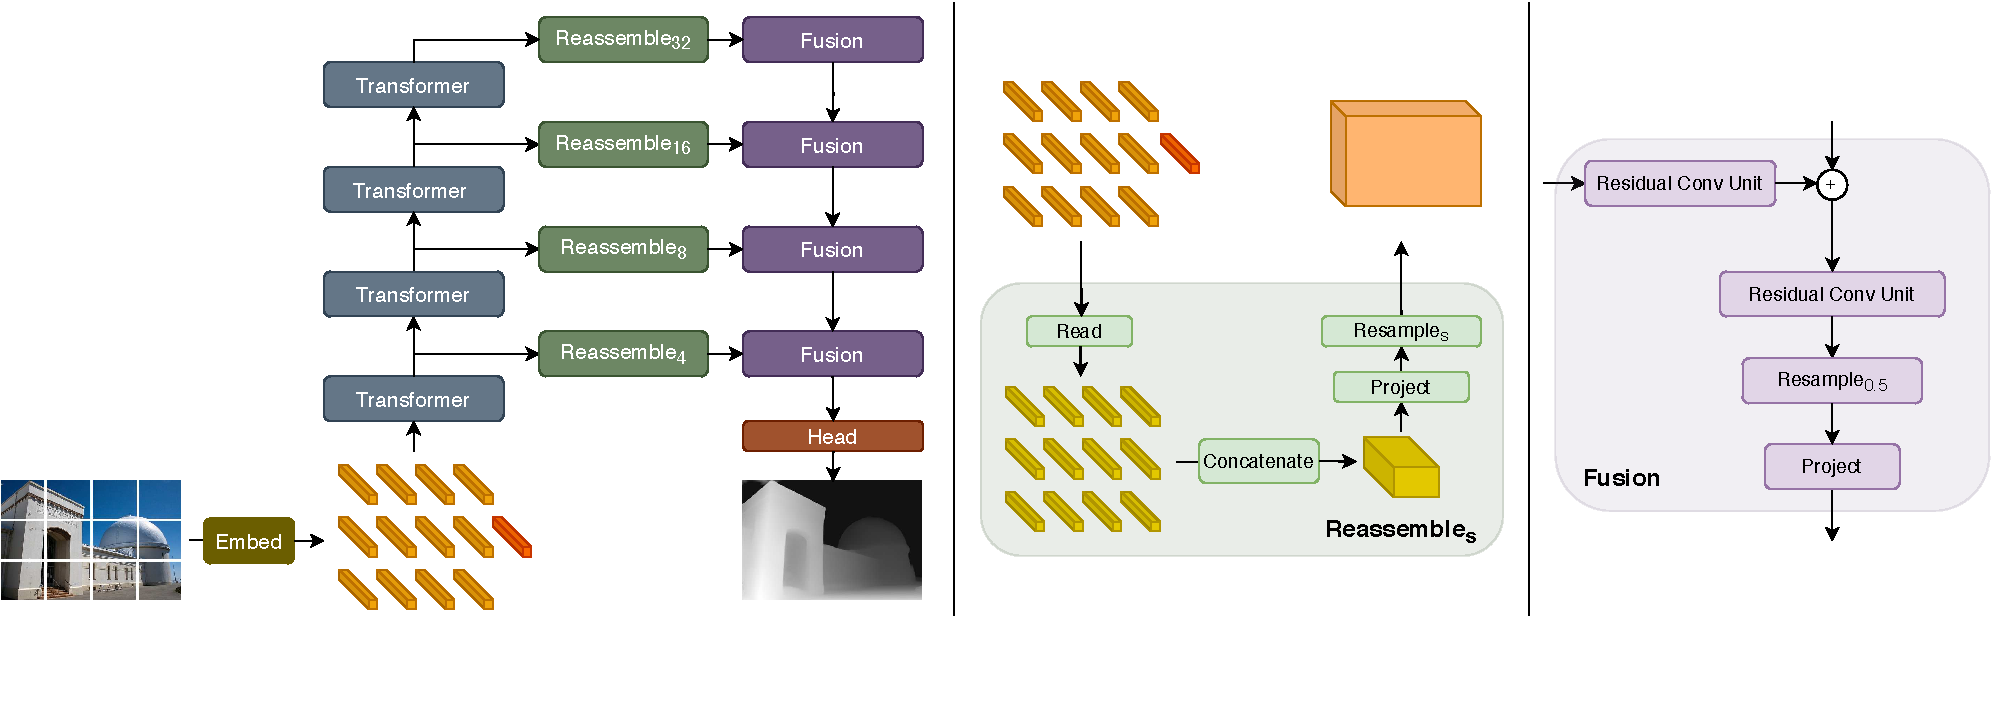
\includegraphics[width=1.0\linewidth,trim={0 16mm 0 0}, clip]{images/diagrams/dense_transformer}
  \vspace{-3.5mm}
  \caption{\emph{Left}: Architecture overview. The input image is transformed
    into tokens (orange) either by extracting non-overlapping patches followed
    by a linear projection of their flattened representation (DPT-Base and
    DPT-Large) or by applying a ResNet-50 feature extractor (DPT-Hybrid). The
    image embedding is augmented with a positional embedding and a
    patch-independent readout token (red) is added. The tokens are passed
    through multiple transformer stages. We reassemble tokens from different
    stages into an image-like representation at multiple resolutions (green).
    Fusion modules (purple) progressively fuse and upsample the representations
    to generate a fine-grained prediction. \emph{Center}: Overview of the
    $\textrm{Reassemble}_{s}$ operation. Tokens are assembled into feature maps
    with $\tfrac{1}{s}$ the spatial resolution of the input image. \emph{Right}:
    Fusion blocks combine features using residual convolutional
    units~\cite{Lin2017} and upsample the feature maps.}
  \label{fig:architecture}
\end{figure*}

This section introduces the dense vision transformer. We maintain the overall
encoder-decoder structure that has been successful for dense prediction in the
past. We leverage vision transformers \cite{Dosovitskiy2020} as the backbone,
show how the representation that is produced by this encoder can be effectively
transformed into dense predictions, and provide intuition for the success of
this strategy. An overview of the complete architecture is shown in
Figure~\ref{fig:architecture}~(left).

\mypara{Transformer encoder.} On a high level, the vision transformer (ViT)
\cite{Dosovitskiy2020} operates on a bag-of-words representation of the image
\cite{Sivic2009}. Image patches that are individually embedded into a feature
space, or alternatively deep features extracted from the image, take the role of
``words''. We will refer to embedded ``words'' as \emph{tokens} throughout the
rest of this work. Transformers transform the set of tokens using sequential
blocks of multi-headed self-attention (MHSA)~\cite{Vaswani2017}, which relate
tokens to each other to transform the representation.

Importantly for our application, a transformer maintains the number of tokens
throughout all computations. Since tokens have a one-to-one correspondence with
image patches, this means that the ViT encoder maintains the spatial resolution
of the initial embedding throughout all transformer stages. Additionally, MHSA
is an inherently global operation, as every token can attend to and thus
influence every other token. Consequently, the transformer has a global
receptive field at every stage after the initial embedding. This is in stark
contrast to convolutional networks, which progressively increase their receptive
field as features pass through consecutive convolution and downsampling layers.

More specifically, ViT extracts a patch embedding from the image by processing
all non-overlapping square patches of size $p^2$ pixels from the image. The
patches are flattened into vectors and individually embedded using a linear
projection. An alternative, more sample-efficient, variant of ViT extracts the
embedding by applying a ResNet50~\cite{He2016} to the image and uses the pixel
features of the resulting feature maps as tokens. Since transformers are
set-to-set functions, they do not intrinsically retain the information of the
spatial positions of individual tokens. The image embeddings are thus
concatenated with a learnable position embedding to add this information to the
representation. Following work in NLP, the ViT additionally adds a special token
that is not grounded in the input image and serves as the final, global image
representation which is used for classification. We refer to this special token
as the \emph{readout} token. The result of applying the embedding procedure to
an image of size $H \times W$ pixels is a a set of
$t^{0} = \{t^{0}_{0}, \dots, t_{N_{p}}^{0}\},\; t_{n}^{0} \in \Re^{D}$ tokens,
where $N_{p} = \frac{HW}{p^{2}}$, $t_{{0}}$ refers to the readout token, and $D$
is the feature dimension of each token.

The input tokens are transformed using $L$ transformer layers into new
representations $t^{l}$, where $l$ refers to the output of the $l$-th
transformer layer. Dosovitskiy \etal~\cite{Dosovitskiy2020} define several
variants of this basic blueprint. We use three variants in our work:
ViT-Base, which uses the patch-based embedding procedure and features 12
transformer layers; ViT-Large, which uses the same embedding procedure and has 24
transformer layers and a wider feature size $D$; and ViT-Hybrid, which employs a
ResNet50 to compute the image embedding followed by 12 transformer layers. We use patch size $p=16$ for all experiments. We refer the
interested reader to the original work~\cite{Dosovitskiy2020} for additional
details on these architectures.

The embedding procedure for ViT-Base and ViT-Large projects the flattened
patches to dimension ${D=768}$ and ${D=1024}$, respectively. Since both feature
dimensions are larger than the number of pixels in an input patch, this means
that the embedding procedure can learn to retain information if it is
beneficial for the task. Features from the input patches can in principle be resolved with
pixel-level accuracy. Similarly, the ViT-Hybrid architecture extracts
features at $\tfrac{1}{16}$ the input resolution, which is twice as high as the lowest-resolution features that are commonly used with convolutional backbones.

\mypara{Convolutional decoder.} Our decoder assembles the set of tokens into
image-like feature representations at various resolutions. The feature
representations are progressively fused into the final dense prediction.
We propose a simple three-stage \emph{Reassemble} operation to recover
image-like representations from the output tokens of arbitrary layers of the
transformer encoder:
\begin{align}
  \textrm{Reassemble}_{s}^{\hat D}(t) = (\textrm{Resample}_{s} \circ \textrm{Concatenate} \circ \textrm{Read})(t),\nonumber
\end{align}
where $s$ denotes the output size ratio of the recovered representation with
respect to the input image, and $\hat D$ denotes the output feature dimension.

We first map the $N_{p}+1$ tokens to a set of $N_{p}$ tokens that is amenable to
spatial concatenation into an image-like representation:
\begin{align}
  \textrm{Read}&: \Re^{N_{p}+1 \times D} \rightarrow  \Re^{N_{p} \times D}.
\end{align}
This operation is essentially responsible for appropriately handling the readout
token. Since the readout token doesn't serve a clear purpose for the task of
dense prediction, but could potentially still be useful to capture and
distribute global information, we evaluate three different variants of this
mapping:
\begin{align}
  \textrm{Read}_{ignore}(t) = \{t_{1}, \dots, t_{N_{p}}\}
\end{align}
simply ignores the readout token,
\begin{align}
  \textrm{Read}_{add}(t) = \{t_{1} + t_{0}, \dots, t_{N_{p}} + t_{0}\}
\end{align}
passes the information from the readout token to all other tokens by adding the
representations, and
\begin{align}
  \textrm{Read}_{proj}(t) = \{\textrm{mlp}(\textrm{cat}(t_{1}, t_{0})), &\dots, \nonumber\\
                                                                        &\textrm{mlp}(\textrm{cat}(t_{N_{p}}, t_{0}))\}
\end{align}
passes information to the other tokens by concatenating the readout to all other
tokens before projecting the representation to the original feature dimension
$D$ using a linear layer followed by a GELU non-linearity \cite{Hendrycks1016}.


After a $\textrm{Read}$ block, the resulting $N_{p}$ tokens can be reshaped into an image-like representation by placing each token according to the position
of the initial patch in the image. Formally, we apply a spatial concatenation
operation that results in a feature map of size
${\tfrac{H}{p} \times \tfrac{W}{p}}$ with $D$ channels:
\begin{align}
  \textrm{Concatenate}&: \Re^{N_p \times D} \rightarrow \Re^{\tfrac{H}{p}  \times \tfrac{W}{p} \times D}.
\end{align}
We finally pass this representation to a spatial resampling layer that scales
the representation to size ${\tfrac{H}{s} \times \tfrac{W}{s}}$ with $\hat D$
features per pixel:
\begin{align}
  \textrm{Resample}_{s}&:  \Re^{\tfrac{H}{p}  \times \tfrac{W}{p} \times D} \rightarrow \Re^{\tfrac{H}{s}  \times \tfrac{W}{s} \times \hat D}.
\end{align}
We implement this operation by first using $1 \times 1$ convolutions to project
the input representation to $\hat D$, followed by a (strided) $3\times 3$ convolution
when $s \geq p$,  or a strided $3 \times 3$ transpose convolution when $s < p$, to
implement spatial downsampling and upsampling operations, respectively.

Irrespective of the exact transformer backbone, we reassemble features at four
different stages and four different resolutions. We assemble features from
deeper layers of the transformer at lower resolution, whereas features from
early layers are assembled at higher resolution. When using ViT-Large, we
reassemble tokens from layers $l =\{5, 12, 18, 24\}$, whereas with ViT-Base we
use layers $l =\{3, 6, 9, 12\}$. We use features from the first and second
ResNet block from the embedding network and stages $l =\{9, 12\}$ when using
ViT-Hybrid. Our default architecture uses projection as the readout operation
and produces feature maps with $\hat D = 256$ dimensions. We will refer to these
architectures as {DPT-Base}, {DPT-Large}, and {DPT-Hybrid}, respectively.

We finally combine the extracted feature maps from consecutive stages using a
RefineNet-based feature fusion block \cite{Lin2017,Xian2018} (see
Figure\ref{fig:architecture} (right)) and progressively upsample the
representation by a factor of two in each fusion stage. The final representation
size has half the resolution of the input image. We attach a task-specific
output head to produce the final prediction. A schematic overview of the
complete architecture is shown in Figure~\ref{fig:architecture}.


\mypara{Handling varying image sizes.} Akin to fully-convolutional networks, DPT
can handle varying image sizes. As long as the image size is divisible by $p$,
the embedding procedure can be applied and will produce a varying number of
image tokens $N_{p}$. As a set-to-set architecture, the transformer encoder can
trivially handle a varying number of tokens. However, the position embedding has
a dependency on the image size as it encodes the locations of the patches in the
input image. We follow the approach proposed in~\cite{Dosovitskiy2020} and
linearly interpolate the position embeddings to the appropriate size. Note that
this can be done on the fly for every image. After the embedding procedure and
the transformer stages, both the reassemble and fusion modules can trivially
handle a varying number of tokens, provided that the input image is aligned to
the stride of the convolutional decoder~($32$ pixels).


\section{Experiments}
We apply DPT to two dense prediction tasks: monocular depth estimation
and semantic segmentation. For both tasks, we show that DPT can significantly
improve accuracy when compared to convolutional networks with a similar
capacity, especially if a large training dataset is available. We first present
our main results using the default configuration and show comprehensive
ablations of different DPT configurations at the end of this section.



\begin{table*}[t!]
  \newcommand{\red}[1] {\small \color{Red}(#1\%)}
  \newcommand{\green}[1] {\small \color{Green}(#1\%)}
  \newcolumntype{d}[1]{D{.}{.}{#1}@{\hspace{1mm}}}
  \newcommand{\oc}[1]{\multicolumn{1}{c}{#1}}
  \newcommand{\dcm}[1]{\multicolumn{2}{c}{#1}}
  \newcommand{\bn}[2]{\multicolumn{1}{B{.}{.}{#1}}{#2}}
  \centering
  \scalebox{0.85}{
    \ra{1.05} \begin{tabular}{@{}l@{\hspace{0mm}}c@{\hspace{3mm}}|@{\hspace{3mm}}d{2.2}l@{\hspace{3.0mm}}d{1.3}c@{\hspace{3.0mm}}d{1.3}c@{\hspace{3.0mm}}d{2.2}c@{\hspace{3.0mm}}d{2.2}c@{\hspace{3.0mm}}d{2.2}c@{}}
      \toprule
                                          & Training set                    & \dcm{DIW}       & \dcm{ETH3D}   & \dcm{Sintel}    & \dcm{KITTI}                 & \dcm{NYU}                   & \dcm{TUM}                                                                                                        \\
                                          &                                 & \dcm{WHDR}      & \dcm{AbsRel}  & \dcm{AbsRel}    & \dcm{$\delta\!\!>\!\!1.25$} & \dcm{$\delta\!\!>\!\!1.25$} & \dcm{$\delta\!\!>\!\!1.25$}                                                                                      \\
                \hline
                DPT - Large               & \small {MIX 6}                  & \bn{2.2}{10.82} & \green{-13.2} & \bn{1.3}{0.089} & \green{-31.2}               & \bn{1.3}{0.270}             & \green{-17.5} & \bn{1.2}{8.46} & \green{-64.6} & \bn{1.2}{8.32} & \green{-12.9} & \bn{1.2}{9.97} & \green{-30.3} \\
                DPT - Hybrid              & \small {MIX 6}                  & 11.06           & \green{-11.2} & 0.093           & \green{-27.6}               & 0.274                       & \green{-16.2} & 11.56           & \green{-51.6} & 8.69          & \green{-9.0}  & 10.89          & \green{-23.2} \\
                MiDaS                     & \small {MIX 6}                  & 12.95           & \red{+3.9}    & 0.116           & \green{-10.5}               & 0.329                       & \red{+0.5}    & 16.08           & \green{-32.7} & 8.71          & \green{-8.8}  & 12.51          & \green{-12.5} \\
                \hline
                MiDaS   \cite{Ranftl2020} & \small {MIX 5}                  & 12.46           &               & 0.129           &                             & 0.327                       &               & 23.90           &               & 9.55          &               & 14.29          &               \\
                \hline
                Li  \cite{LiSnavely2018}  & \small MD  \cite{LiSnavely2018} & 23.15           &               & 0.181           &                             & 0.385                       &               & 36.29           &               & 27.52         &               & 29.54          &               \\
                Li \cite{Li2019}          & \small MC  \cite{Li2019}        & 26.52           &               & 0.183           &                             & 0.405                       &               & 47.94           &               & 18.57         &               & 17.71          &               \\
                Wang \cite{Wang2019}      & \small WS   \cite{Wang2019}     & 19.09           &               & 0.205           &                             & 0.390                       &               & 31.92           &               & 29.57         &               & 20.18          &               \\
                Xian  \cite{Xian2018}     & \small RW   \cite{Xian2018}     & 14.59           &               & 0.186           &                             & 0.422                       &               & 34.08           &               & 27.00         &               & 25.02          &               \\
                Casser \cite{Casser2019}  & \small CS   \cite{Cordts2016}   & 32.80           &               & 0.235           &                             & 0.422                       &               & 21.15           &               & 39.58         &               & 37.18          &               \\
                \bottomrule
              \end{tabular}
            } \vspace{1.5mm}
            \caption{Comparison to the state of the art on monocular depth
              estimation. We evaluate zero-shot cross-dataset transfer according
              to the protocol defined in \cite{Ranftl2020}. Relative performance is computed with respect to the original MiDaS model
              \cite{Ranftl2020}. Lower is better for all metrics.}
            \label{tab:mono_sota}
          \end{table*}

\begin{table}[b!]
  \centering \scalebox{0.80}{
    \ra{1.05} \begin{tabular}{@{}l@{\hspace{3mm}}c@{\hspace{3mm}}c@{\hspace{3mm}}c@{\hspace{3mm}}c@{\hspace{3mm}}c@{\hspace{3mm}}c@{\hspace{3mm}}c@{}}
                \toprule
                                   & {$\delta\!\!>\!\!1.25$} & {$\delta\!\!>\!\!1.25^{2}$} & {$\delta\!\!>\!\!1.25^{3}$} & AbsRel    & RMSE      & log10     \\
                \midrule
                DORN \cite{Fu2018} & 0.828                   & 0.965                       & 0.992                       & 0.115     & 0.509     & 0.051     \\
                VNL \cite{Yin2019} & 0.875                   & 0.976                       & 0.994                       & 0.111     & 0.416     & 0.048     \\
                BTS \cite{Lee2019} & 0.885                   & 0.978                       & 0.994                       & \bf 0.110 & 0.392     & 0.047     \\
                \midrule
                DPT-Hybrid         & \bf 0.904               & \bf 0.988                   & \bf 0.998                   & \bf 0.110 & \bf 0.357 & \bf 0.045 \\
                \bottomrule
                \end{tabular}
                }
            \caption{Evaluation on NYUv2 depth. }
            \label{tab:mono_nyuv2}
          \end{table}

\begin{table}[b!]
  \centering \scalebox{0.76}{
    \ra{1.05} \begin{tabular}{@{}l@{\hspace{3mm}}c@{\hspace{3mm}}c@{\hspace{3mm}}c@{\hspace{3mm}}c@{\hspace{3mm}}c@{\hspace{3mm}}c@{\hspace{3mm}}c@{}}
                \toprule
                                   & {$\delta\!\!>\!\!1.25$} & {$\delta\!\!>\!\!1.25^{2}$} & {$\delta\!\!>\!\!1.25^{3}$} & AbsRel    & RMSE       & RMSE log  \\
                \midrule
                DORN \cite{Fu2018} & 0.932                   & 0.984                       & 0.994                       & 0.072     & 2.626      & 0.120     \\
                VNL \cite{Yin2019} & 0.938                   & 0.990                       & 0.998                       & 0.072     & 3.258      & 0.117     \\
                BTS \cite{Lee2019} & 0.956                   & 0.993                       & 0.998                       & \bf 0.059 & 2.756      & 0.096 \\
                \midrule
                DPT-Hybrid         & \bf 0.959               & \bf 0.995                   & \bf 0.999                   & 0.062     & \bf  2.573 & \bf 0.092     \\
                \bottomrule
                \end{tabular}
                }
            \caption{Evaluation on KITTI (Eigen split). }
            \label{tab:mono_kitti}
          \end{table}


\subsection{Monocular Depth Estimation}
Monocular depth estimation is typically cast as a dense regression problem.
It has been shown that massive meta-datasets can be constructed from existing
sources of data, provided that some care is taken in how different
representations of depth are unified into a common representation and that
common ambiguities (such as scale ambiguity) are appropriately handled in the
training loss \cite{Ranftl2020}. Since transformers are known to realize their
full potential only when an abundance of training data is available, monocular
depth estimation is an ideal task to test the capabilities of DPT.

\mypara{Experimental protocol.} We closely follow the protocol of Ranftl
\etal\cite{Ranftl2020}. We learn a monocular depth prediction network using a
scale- and shift-invariant trimmed loss that operates on an inverse depth
representation, together with the gradient-matching loss proposed
in~\cite{LiSnavely2018}. We construct a meta-dataset that includes the original
datasets that were used in \cite{Ranftl2020} (referred to as \emph{MIX 5} in
that work) and extend it with with five additional datasets
(\cite{Xian2020,Yao2020,tartanair2020,Huang2020,irs2020}). We refer to this
meta-dataset as \emph{MIX 6}. It contains about 1.4 million images and is, to
the best of our knowledge, the largest training set for monocular depth
estimation that has ever been compiled.

We use multi-objective optimization \cite{Sener2018} together with Adam
\cite{Kingma2015} and set a learning rate of $1\mathrm{e-}5$ for the backbone
and $1\mathrm{e-}4$ for the decoder weights. The encoder is initialized with
ImageNet-pretrained weights, whereas the decoder is initialized randomly. We use
an output head that consists of 3 convolutional layers. The output head
progressively halves the feature dimension and upsamples the predictions to the
input resolution after the first convolutional layer (details in supplementary
material). We disable batch normalization in the decoder, as we found it to
negatively influence results for regression tasks. We resize the image such that
the longer side is $384$ pixels and train on random square crops of size $384$.
We train for $60$ epochs, where one epoch consists of $72@000$ steps with a
batch size of $16$. As the batch size is not divisible by the number of
datasets, we construct a mini-batch by first drawing datasets uniformly at
random before sampling from the respective datasets. We perform random
horizontal flips for data augmentation. Similar to \cite{Ranftl2020}, we first
pretrain on a well-curated subset of the data \cite{Xian2020,Xian2018,Yao2020}
for $60$ epochs before training on the full dataset.


\mypara{Zero-shot cross-dataset transfer.} Table~\ref{tab:mono_sota} shows
the results of zero-shot transfer to different datasets that were not seen during training. We refer the
interested reader to Ranftl \etal\cite{Ranftl2020} for details of the evaluation procedure
and error metrics. For all metrics, lower is better. Both DPT
variants significantly outperform the state of the art. The average relative
improvement over the best published architecture, MiDaS, is more than
23\% for DPT-Hybrid and 28\% for DPT-Large. DPT-Hybrid achieves this with a
comparable network capacity (Table~\ref{tab:inference_time}), while
DPT-Large is about $3$ times larger than MiDaS. Note that both architectures
have similar latency to MiDaS~(Table \ref{tab:inference_time}).

To ensure that the observed improvements are not only due to the enlarged
training set, we retrain the fully-convolutional network used by MiDaS on our
larger meta-dataset \emph{MIX 6}. While the fully-convolutional network indeed
benefits from the larger training set, we observe that both DPT variants still
strongly outperform this network. This shows that DPT can better benefit from
increased training set size, an observation that matches previous findings on
transformer-based architectures in other fields.

The quantitative results are supported by visual comparisons in
Figure~\ref{fig:monodepth_comparison}. DPT can better reconstruct fine details
while also improving global coherence in areas that are challenging for the
convolutional architecture (for example, large homogeneous regions or relative
depth arrangement across the image).


\begin{figure*}
  \centering \def\mywidth{0.24}
  \begin{tabular}{@{}c@{\hspace{1mm}}c@{\hspace{1mm}}c@{\hspace{1mm}}c@{\hspace{1mm}}c@{}}
    Input & MiDaS (MIX 6) & DPT-Hybrid & DPT-Large\\
    \adjincludegraphics[width=\mywidth\linewidth,trim={0 0 0 0},clip]{images/monodepth/input/586_c9afe6fbc2b9eee84adbf639eb0629a0a4b4be51} &
    \adjincludegraphics[width=\mywidth\linewidth,trim={0 0 0 0},clip]{images/monodepth/midas_2.1/586_c9afe6fbc2b9eee84adbf639eb0629a0a4b4be51} &
    \adjincludegraphics[width=\mywidth\linewidth,trim={0 0 0 0},clip]{images/monodepth/dpt_rn50/586_c9afe6fbc2b9eee84adbf639eb0629a0a4b4be51} &
    \adjincludegraphics[width=\mywidth\linewidth,trim={0 0 0 0},clip]{images/monodepth/dpt_large/586_c9afe6fbc2b9eee84adbf639eb0629a0a4b4be51} \\

    \adjincludegraphics[width=\mywidth\linewidth,trim={0 0 0 0},clip]{images/monodepth/input/317_bb78c3e55df7407c449a72f3e6833a20d5742b1d} &
    \adjincludegraphics[width=\mywidth\linewidth,trim={0 0 0 0},clip]{images/monodepth/midas_2.1/317_bb78c3e55df7407c449a72f3e6833a20d5742b1d} &
    \adjincludegraphics[width=\mywidth\linewidth,trim={0 0 0 0},clip]{images/monodepth/dpt_rn50/317_bb78c3e55df7407c449a72f3e6833a20d5742b1d} &
    \adjincludegraphics[width=\mywidth\linewidth,trim={0 0 0 0},clip]{images/monodepth/dpt_large/317_bb78c3e55df7407c449a72f3e6833a20d5742b1d} \\
    \adjincludegraphics[width=\mywidth\linewidth,trim={0 0 0 0},clip]{images/monodepth/input/00022_00197_outdoor_300_050} &
    \adjincludegraphics[width=\mywidth\linewidth,trim={0 0 0 0},clip]{images/monodepth/midas_2.1/00022_00197_outdoor_300_050} &
    \adjincludegraphics[width=\mywidth\linewidth,trim={0 0 0 0},clip]{images/monodepth/dpt_rn50/00022_00197_outdoor_300_050} &
    \adjincludegraphics[width=\mywidth\linewidth,trim={0 0 0 0},clip]{images/monodepth/dpt_large/00022_00197_outdoor_300_050} \\
  \end{tabular}
  \caption{Sample results for monocular depth estimation. Compared to the fully-convolutional network used by MiDaS, DPT shows better global coherence
    (e.g., sky, second row) and finer-grained details (e.g., tree branches, last row).} %
\label{fig:monodepth_comparison}
\end{figure*}

\mypara{Fine-tuning on small datasets.} We fine-tune DPT-Hybrid on the KITTI
\cite{Geiger2012} and NYUv2 \cite{Silberman2012} datasets to further
compare the representational power of DPT to existing work. Since the network was trained
with an affine-invariant loss, its predictions are arbitrarily scaled and
shifted and can have large magnitudes. Direct fine-tuning would
thus be challenging, as the global mismatch in the magnitude of the predictions to
the ground truth would dominate the loss. We thus first align predictions of the
initial network to each training sample using the robust alignment procedure
described in \cite{Ranftl2020}. We then average the resulting scales and shifts
across the training set and apply the average scale and shift to the predictions
before passing the result to the loss. We fine-tune with the loss
proposed by Eigen~\etal~\cite{Eigen2014}. We disable the gradient-matching loss
for KITTI since this dataset only provides sparse ground truth.


Tables \ref{tab:mono_nyuv2} and \ref{tab:mono_kitti} summarize the results. Our
architecture matches or improves state-of-the-art performance on both
datasets in all metrics. This indicates that DPT can also be usefully applied to smaller datasets.


\subsection{Semantic Segmentation}

We choose semantic segmentation as our second task since it is representative
of discrete labeling tasks and is a very competitive proving ground for dense
prediction architectures. We employ the same backbone and decoder structure as
in previous experiments. We use an output head that predicts at half resolution
and upsamples the logits to full resolution using bilinear interpolation
(details in supplementary material). The encoder is again initialized from
ImageNet-pretrained weights, and the decoder is initialized randomly.


\mypara{Experimental protocol.} We closely follow the protocol established by
Zhang~\etal~\cite{Zhang2020}. We employ a cross-entropy loss and add an
auxiliary output head together with an auxiliary loss to the output of the
penultimate fusion layer. We set the weight of the auxiliary loss to $0.2$.
Dropout with a rate of $0.1$ is used before the final classification layer in
both heads. We use SGD with momentum $0.9$ and a polynomial learning rate
scheduler with decay factor $0.9$. We use batch normalization in the fusion
layers and train with batch size $48$. Images are resized to $520$ pixels side
length. We use random horizontal flipping and random rescaling in the range
$\in (0.5, 2.0)$ for data augmentation. We train on square random crops of size
$480$. We set the learning rate to $0.002$. We use multi-scale inference at test
time and report both pixel accuracy (pixAcc) as well as mean
Intersection-over-Union (mIoU).

\begin{figure*}[!t]
  \centering
  \def\mywidth{0.24}
  \begin{tabular}{@{}l@{\hspace{1mm}}c@{\hspace{1mm}}c@{\hspace{1mm}}c@{\hspace{1mm}}c@{}}
    \parbox[t]{2.2mm}{\rotatebox[origin=c,x=0mm,y=3.0mm]{90}{\small ResNeSt-200 \cite{Zhang2020}}}
    &
    \adjincludegraphics[width=\mywidth\linewidth,trim={0 0 0 0},clip]{images/segmentations/ade20k/resnest200_inset/ADE_val_00000053_overlay} &
    \adjincludegraphics[width=\mywidth\linewidth,trim={0 0 0 1.50cm},clip]{images/segmentations/ade20k/resnest200/ADE_val_00000073} &
    \adjincludegraphics[width=\mywidth\linewidth,trim={0 0 0 0},clip]{images/segmentations/pcontext/resnest200_inset/2008_000123_overlay} &
    \adjincludegraphics[width=\mywidth\linewidth,trim={0 0 0 1.47cm},clip]{images/segmentations/pcontext/resnest200/2008_000194} \\
    \parbox[t]{2.2mm}{\rotatebox[origin=c,x=0mm,y=5.8mm]{90}{\small DPT-Hybrid}}
    &
    \adjincludegraphics[width=\mywidth\linewidth,trim={0 0 0 0},clip]{images/segmentations/ade20k/dpt_hybrid_inset/ADE_val_00000053_overlay} &
    \adjincludegraphics[width=\mywidth\linewidth,trim={0 0 0 1.50cm},clip]{images/segmentations/ade20k/dpt_hybrid/ADE_val_00000073} &
    \adjincludegraphics[width=\mywidth\linewidth,trim={0 0 0 0},clip]{images/segmentations/pcontext/dpt_hybrid_inset/2008_000123_overlay} &
    \adjincludegraphics[width=\mywidth\linewidth,trim={0 0 0 1.47cm},clip]{images/segmentations/pcontext/dpt_hybrid/2008_000194} \\
  \end{tabular}
  \caption{Sample results for semantic segmentation on ADE20K (first and second column) and Pascal Context (third and fourth column). Predictions are frequently better aligned
to object edges and less cluttered.}
\label{fig:seg_comparison}
\end{figure*}

\mypara{ADE20K.} We train the DPT on the ADE20K semantic segmentation dataset
\cite{Zhou2017} for $240$ epochs. Table~\ref{tab:ade20k} summarizes our results
on the validation set. DPT-Hybrid outperforms all existing fully-convolutional
architectures. DPT-Large performs slightly worse, likely because of the
significantly smaller dataset compared to our previous experiments. Figure
\ref{fig:seg_comparison} provides visual comparisons. We observe that the DPT
tends to produce cleaner and finer-grained delineations of object boundaries and
that the predictions are also in some cases less cluttered.

\mypara{Fine-tuning on smaller datasets.} We fine-tune DPT-Hybrid on the Pascal
Context dataset~\cite{Mottaghi2014} for 50 epochs. All other hyper-parameters
remain the same. Table~\ref{tab:pcontext} shows results on the validation set
for this experiment. We again see that DPT can provide strong performance even
on smaller datasets.

\begin{table}[b]
  \centering
  \scalebox{0.85}{
  \ra{1.05}
    \begin{tabular}{@{}l@{\hspace{3.5mm}}cl@{\hspace{5mm}}c@{\hspace{5mm}}c@{}}
     \toprule
                & Backbone   & & pixAcc [\%] & mIoU [\%]  \\
     \midrule
     OCNet      & ResNet101  & \cite{Yuan2020}  & --          & 45.45      \\
     ACNet      & ResNet101  & \cite{Fu2019} & 81.96       & 45.90      \\
     DeeplabV3  & ResNeSt-101& \cite{Zhang2020,Chen2017} & 82.07       & 46.91      \\
     DeeplabV3  & ResNeSt-200& \cite{Zhang2020,Chen2017} & 82.45       & 48.36      \\
     \midrule
     DPT-Hybrid & ViT-Hybrid & & \bf{83.11}  & \bf{49.02} \\
     DPT-Large  & ViT-Large &  & 82.70 & 47.63           \\
     \bottomrule
    \end{tabular}
  }
  \vspace{1.5mm}
   \caption{Semantic segmentation results on the ADE20K validation set.}
   \label{tab:ade20k}
\end{table}

\begin{table}[b]
  \centering
  \scalebox{0.85}{
  \ra{1.05}
    \begin{tabular}{@{}l@{\hspace{3.5mm}}cl@{\hspace{5mm}}c@{\hspace{5mm}}c@{}}
     \toprule
                & Backbone    &                           & pixAcc [\%] & mIoU [\%] \\
     \midrule
     OCNet      & HRNet-W48   & \cite{Yuan2020,Wang2020}  & --          & 56.2      \\
     DeeplabV3  & ResNeSt-200 & \cite{Zhang2020,Chen2017} & 82.50       & 58.37     \\
     DeeplabV3  & ResNeSt-269 & \cite{Zhang2020,Chen2017} & 83.06       & 58.92     \\
     \midrule
     DPT-Hybrid & ViT-Hybrid  &                           & \bf 84.83       & \bf 60.46     \\
     \bottomrule
    \end{tabular}
    }
   \caption{Finetuning results on the Pascal Context validation set.}
   \label{tab:pcontext}
\end{table}


\subsection{Ablations}
We examine a number of aspects and technical choices in DPT via ablation
studies. We choose monocular depth estimation as the task for our ablations and
follow the same protocol and hyper-parameter settings as previously described.
We use a reduced meta-dataset that is composed of three
datasets~\cite{Xian2018,Xian2020,Yao2020} and consists of about $41@000$ images.
We choose these datasets since they provide high-quality ground truth. We split
each dataset into a training set and a small validation set of about $1@000$ images
total. We report results on
the validation sets in terms of relative absolute deviation after affine
alignment of the predictions to the ground truth \cite{Ranftl2020}. Unless
specified otherwise, we use ViT-Base as the backbone architecture.

\mypara{Skip connections.} Convolutional architectures offer natural points of
interest for passing features from the encoder to the decoder, namely before or after
downsampling of the representation. Since the transformer backbone maintains a
constant feature resolution, it is not clear at which points in the backbone
features should be tapped. We evaluate several possible choices in
Table~\ref{tab:ablation_skipconnections} (top). We observe that it is beneficial to
tap features from layers that contain low-level features as well as
deeper layers that contain higher-level features. We adopt the best setting for
all further experiments.

We perform a similar experiment with the hybrid architecture in
Table~\ref{tab:ablation_skipconnections} (bottom), where R0 and R1 refer to
using features from the first and second downsampling stages of the ResNet50
embedding network. We observe that using low-level features from the embedding
network leads to better performance than using features solely from
the transformer stages. We use this setting for all further experiments that
involve the hybrid architecture.

\begin{table}[b]
  \centering
  \scalebox{0.85}{
  \ra{1.05}
  \renewcommand{\arraystretch}{1.2}
  \begin{tabular}{@{}c|c@{\hspace{3mm}}|c@{\hspace{2mm}}c@{\hspace{2mm}}c|@{\hspace{2mm}}r@{}}
     \toprule
                                                                               & Layer $l$     & HRWSI      & BlendedMVS & ReDWeb     & Mean       \\
      \hline
     \parbox[t]{2mm}{\multirow{3}{*}{\rotatebox[origin=c]{90}{\small Base}}}   & \{3, 6, 9, 12\}   & 0.0793     & 0.0780     & 0.0892     & 0.0822     \\
                                                                               & \{6, 8, 10, 12\}  & 0.0801     & 0.0789     & 0.0904     & 0.0831     \\
                                                                               & \{9, 10, 11, 12\} & 0.0805     & 0.0766     & 0.0912     & 0.0828     \\
     \hline
     \parbox[t]{2mm}{\multirow{2}{*}{\rotatebox[origin=c]{90}{\small Hybrid}}} & \{3, 6, 9, 12\}   & 0.0747     & \bf 0.0748 & 0.0865     & 0.0787     \\
                                                                               & \{R0, R1, 9, 12\} & \bf 0.0742 & 0.0751     & \bf 0.0857 & \bf 0.0733 \\
     \bottomrule
    \end{tabular}
  }
  \caption{Performance of attaching skip connections to different encoder layers. Best results are achieved with a combination of
  skip connections from shallow and deep layers.}
   \label{tab:ablation_skipconnections}
\end{table}

\mypara{Readout token.} Table~\ref{tab:ablation_readout} examines various choices
for implementing the first stage of the \emph{Reassemble} block to handle the
readout token. While ignoring the token yields good performance, projection
provides slightly better performance on average. Adding the token, on the other
hand, yields worse performance than simply ignoring it. We use
projection for all further experiments.


\begin{table}[t]
  \centering
  \scalebox{0.85}{
  \ra{1.05}
    \begin{tabular}{@{}l|@{\hspace{3mm}}c@{\hspace{2mm}}c@{\hspace{2mm}}c|@{\hspace{2mm}}r@{}}
     \toprule
              & HRWSI      & BlendedMVS & ReDWeb     & Mean       \\
      \hline
      Ignore  & \bf 0.0793 & 0.0780     & \bf 0.0892 & 0.0822     \\
      Add     & 0.0799     & 0.0789     & 0.0904     & 0.0831     \\
      Project & 0.0797     & \bf 0.0764 & 0.0895     & \bf 0.0819 \\
      \bottomrule
    \end{tabular}
  }
  \vspace{1.5mm}
  \caption{
    Performance of approaches to handle the readout token. Fusing the readout token
    to the individual input tokens using a projection layer yields the best performance.
  }
   \label{tab:ablation_readout}
\end{table}
\begin{table}[b]
  \centering
  \scalebox{0.85}{
  \ra{1.05}
    \begin{tabular}{@{}l@{\hspace{3mm}}c@{\hspace{2mm}}c@{\hspace{2mm}}c|@{\hspace{2mm}}r@{}}
     \toprule
                     & HRWSI      & BlendedMVS & ReDWeb     & Mean       \\
      \hline
      ResNet50       & 0.0890     & 0.0887     & 0.1029     & 0.0935     \\
      ResNext101-WSL & 0.0780     & 0.0751     & 0.0886     & 0.0806     \\
      \hline
      DeIT-Base      & 0.0798     & 0.0804     & 0.0925     & 0.0842     \\
      DeIT-Base-Dist & 0.0758     & 0.0758     & 0.0871     & 0.0796     \\
      \hline
      ViT-Base       & 0.0797     & 0.0764     & 0.0895     & 0.0819     \\
      ViT-Large      & 0.0740     & 0.0747     & \bf 0.0846 & \bf 0.0778 \\
      ViT-Hybrid     & \bf 0.0738 & \bf 0.0746 & 0.0864     & 0.0783     \\
      \bottomrule
    \end{tabular}
  }
  \vspace{1.5mm}
  \caption{Ablation of backbones. The hybrid and large backbones
    consistently outperform the convolutional baselines. The base architecture
    can outperform the convolutional baseline with better pretraining (DeIT-Base-Dist).
  }
   \label{tab:ablation_backbones}
\end{table}



\mypara{Backbones.} The performance of different backbones is shown in
Table~\ref{tab:ablation_backbones}. ViT-Large outperforms all other backbones
but is also almost three times larger than ViT-Base and ViT-Hybrid. ViT-Hybrid
outperforms ViT-Base with a similar number of parameters
and has comparable performance to the large backbone. As such it
provides a good trade-off between accuracy and capacity.


ViT-Base has comparable performance to ResNext101-WSL, while ViT-Hybrid and
ViT-Large improve performance even though they have been pretrained on
significantly less data. Note that ResNext101-WSL was pretrained on a
billion-scale corpus of weakly supervised data~\cite{Mahajan2018} in addition to
ImageNet pretraining. It has been observed that this pretraining boosts the
performance of monocular depth prediction \cite{Ranftl2020}. This
architecture corresponds to the original MiDaS architecture.

We finally compare to a recent variant of ViT called
DeIT~\cite{touvron2020deit}. DeIT trains the ViT architecture with a more
data-efficient pretraining procedure. Note that the DeIT-Base architecture is
identical to ViT-Base, while DeIT-Base-Dist introduces an additional
\textit{distillation} token, which we ignore in the Reassemble operation. We observe
that DeIT-Base-Dist indeed improves performance when compared to ViT-Base. This
indicates that similarly to convolutional architectures, improvements in
pretraining procedures for image classification can benefit dense prediction
tasks.

\mypara{Inference resolution.} While fully-convolutional architectures can have
large effective receptive fields in their deepest layers, the layers close to
the input are local and have small receptive fields. Performance thus suffers
heavily when performing inference at an input resolution that is significantly
different from the training resolution. Transformer encoders, on the other hand,
have a global receptive field in every layer. We conjecture that this makes DPT
less dependent on inference resolution. To test this hypothesis, we plot the
loss in performance of different architectures when performing inference at
resolutions higher than the training resolution of $384 \times 384$ pixels. We
plot the relative decrease in performance in percent with respect to the
performance of performing inference at the training resolution in
Figure~\ref{fig:inference_resolution}. We observe that the performance of DPT variants indeed degrades more gracefully as inference resolution increases.

\begin{figure}[t!]
  \centering
  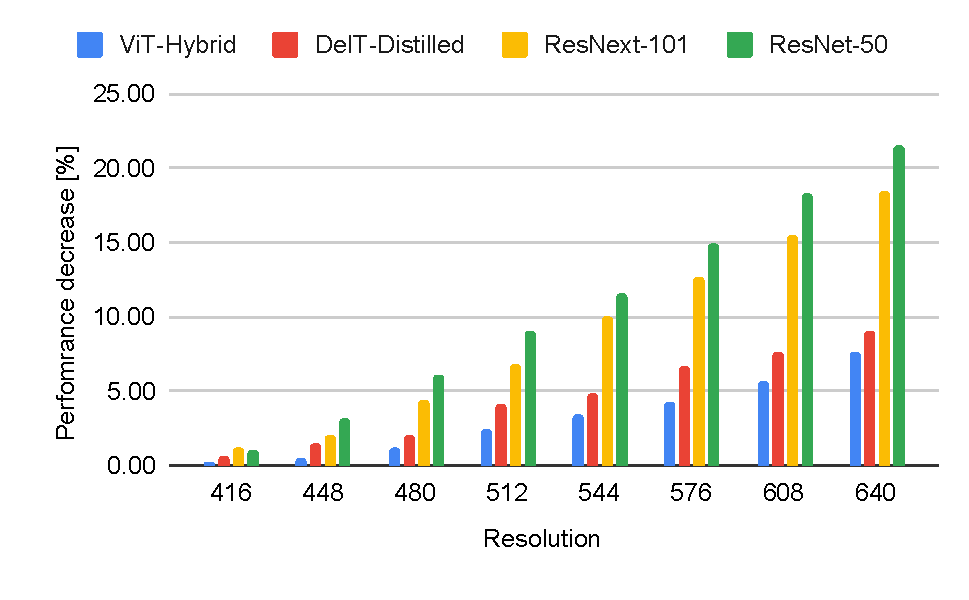
\includegraphics[width=0.90\linewidth,trim={9mm 8mm 9mm 5mm},clip]{images/other/size_dependence}
  \caption{Relative loss in performance for different inference resolutions (lower is better).
  }
  \label{fig:inference_resolution}
\end{figure}

\mypara{Inference speed.} Table \ref{tab:inference_time} shows inference time
for different network architectures. Timings were conducted on an Intel Xeon
Platinum 8280 CPU @ 2.70GHz with 8 physical cores and an Nvidia RTX 2080 GPU.
We use square images with a width of $384$ pixels and report the average over $400$ runs.
DPT-Hybrid and DPT-Large show comparable latency to the fully-convolutional
architecture used by MiDaS. Interestingly, while DPT-Large is substantially
larger than the other architectures in terms of parameter count, it has
competitive latency since it exposes a high degree of parallelism through its
wide and comparatively shallow structure.

\begin{table}[htb!]
  \centering
  \scalebox{0.82}{
  \ra{1.05}
    \begin{tabular}{@{}l@{\hspace{3mm}}c@{\hspace{3mm}}c@{\hspace{3mm}}c@{\hspace{3mm}}c@{}}
     \toprule
      & MiDaS  & DPT-Base & DPT-Hybrid & DPT-Large \\
      \midrule
      Parameters [million] &  105 & 112 &  123 & 343 \\
      Time [ms] &  32 & 17 & 38 & 35\\
      \bottomrule
    \end{tabular}
  }
  \caption{Model statistics. DPT
  has comparable inference speed to the state of the art.}
   \label{tab:inference_time}
 \end{table}


\section{Conclusion}
We have introduced the dense prediction transformer, DPT, a neural network
architecture that effectively leverages vision transformers for dense prediction
tasks. Our experiments on monocular depth estimation and semantic segmentation
show that the presented architecture produces more fine-grained and globally
coherent predictions when compared to fully-convolutional architectures. Similar
to prior work on transformers, DPT unfolds its full potential when trained on
large-scale datasets.

{\small \bibliographystyle{ieee_fullname} \bibliography{egbib} }

\newpage

\appendix

\renewcommand{\thefigure}{A\arabic{figure}}
\renewcommand{\theHfigure}{A\arabic{figure}}
\setcounter{figure}{0}

\renewcommand{\thetable}{A\arabic{table}}
\renewcommand{\theHtable}{A\arabic{table}}
\setcounter{table}{0}



\twocolumn[
\vspace{1cm}
\begin{center}
\section*{\LARGE Supplementary Material}
\end{center}
\vspace{2cm}
]


\section{Architecture details}
We provide additional technical details in this section.
\begin{figure*}[t]
    \begin{tabular}{@{}c@{\hspace{13mm}}c@{\hspace{13mm}}c@{}}
    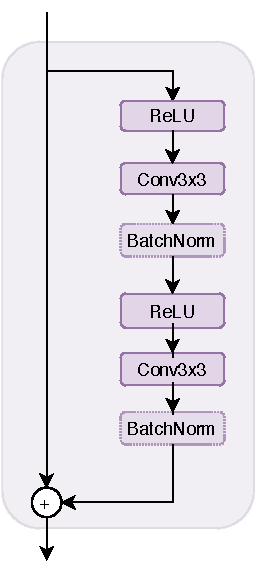
\includegraphics[height=4.5cm]{images/diagrams/resiconv} &
    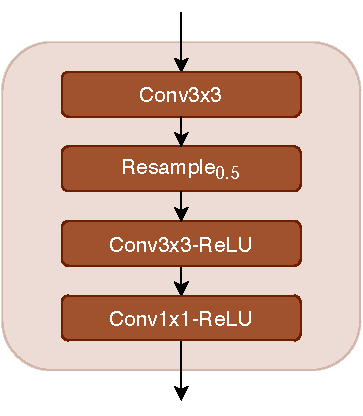
\includegraphics[width=0.23\linewidth]{images/diagrams/monodepth_head} &
    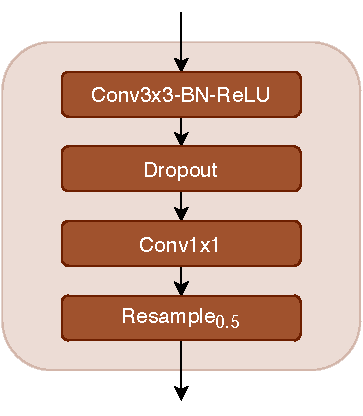
\includegraphics[width=0.23\linewidth]{images/diagrams/segmentation_head} \\
    \small (a) Residual Convolutional Unit \cite{Lin2017} & \small (b) Monocular depth estimation head & \small (c) Semantic segmentation head
  \end{tabular}
  \caption{Schematics of different architecture blocks.}
  \label{fig:archdetails}
\end{figure*}

\begin{figure*}[b]
  \centering
  \fbox{
    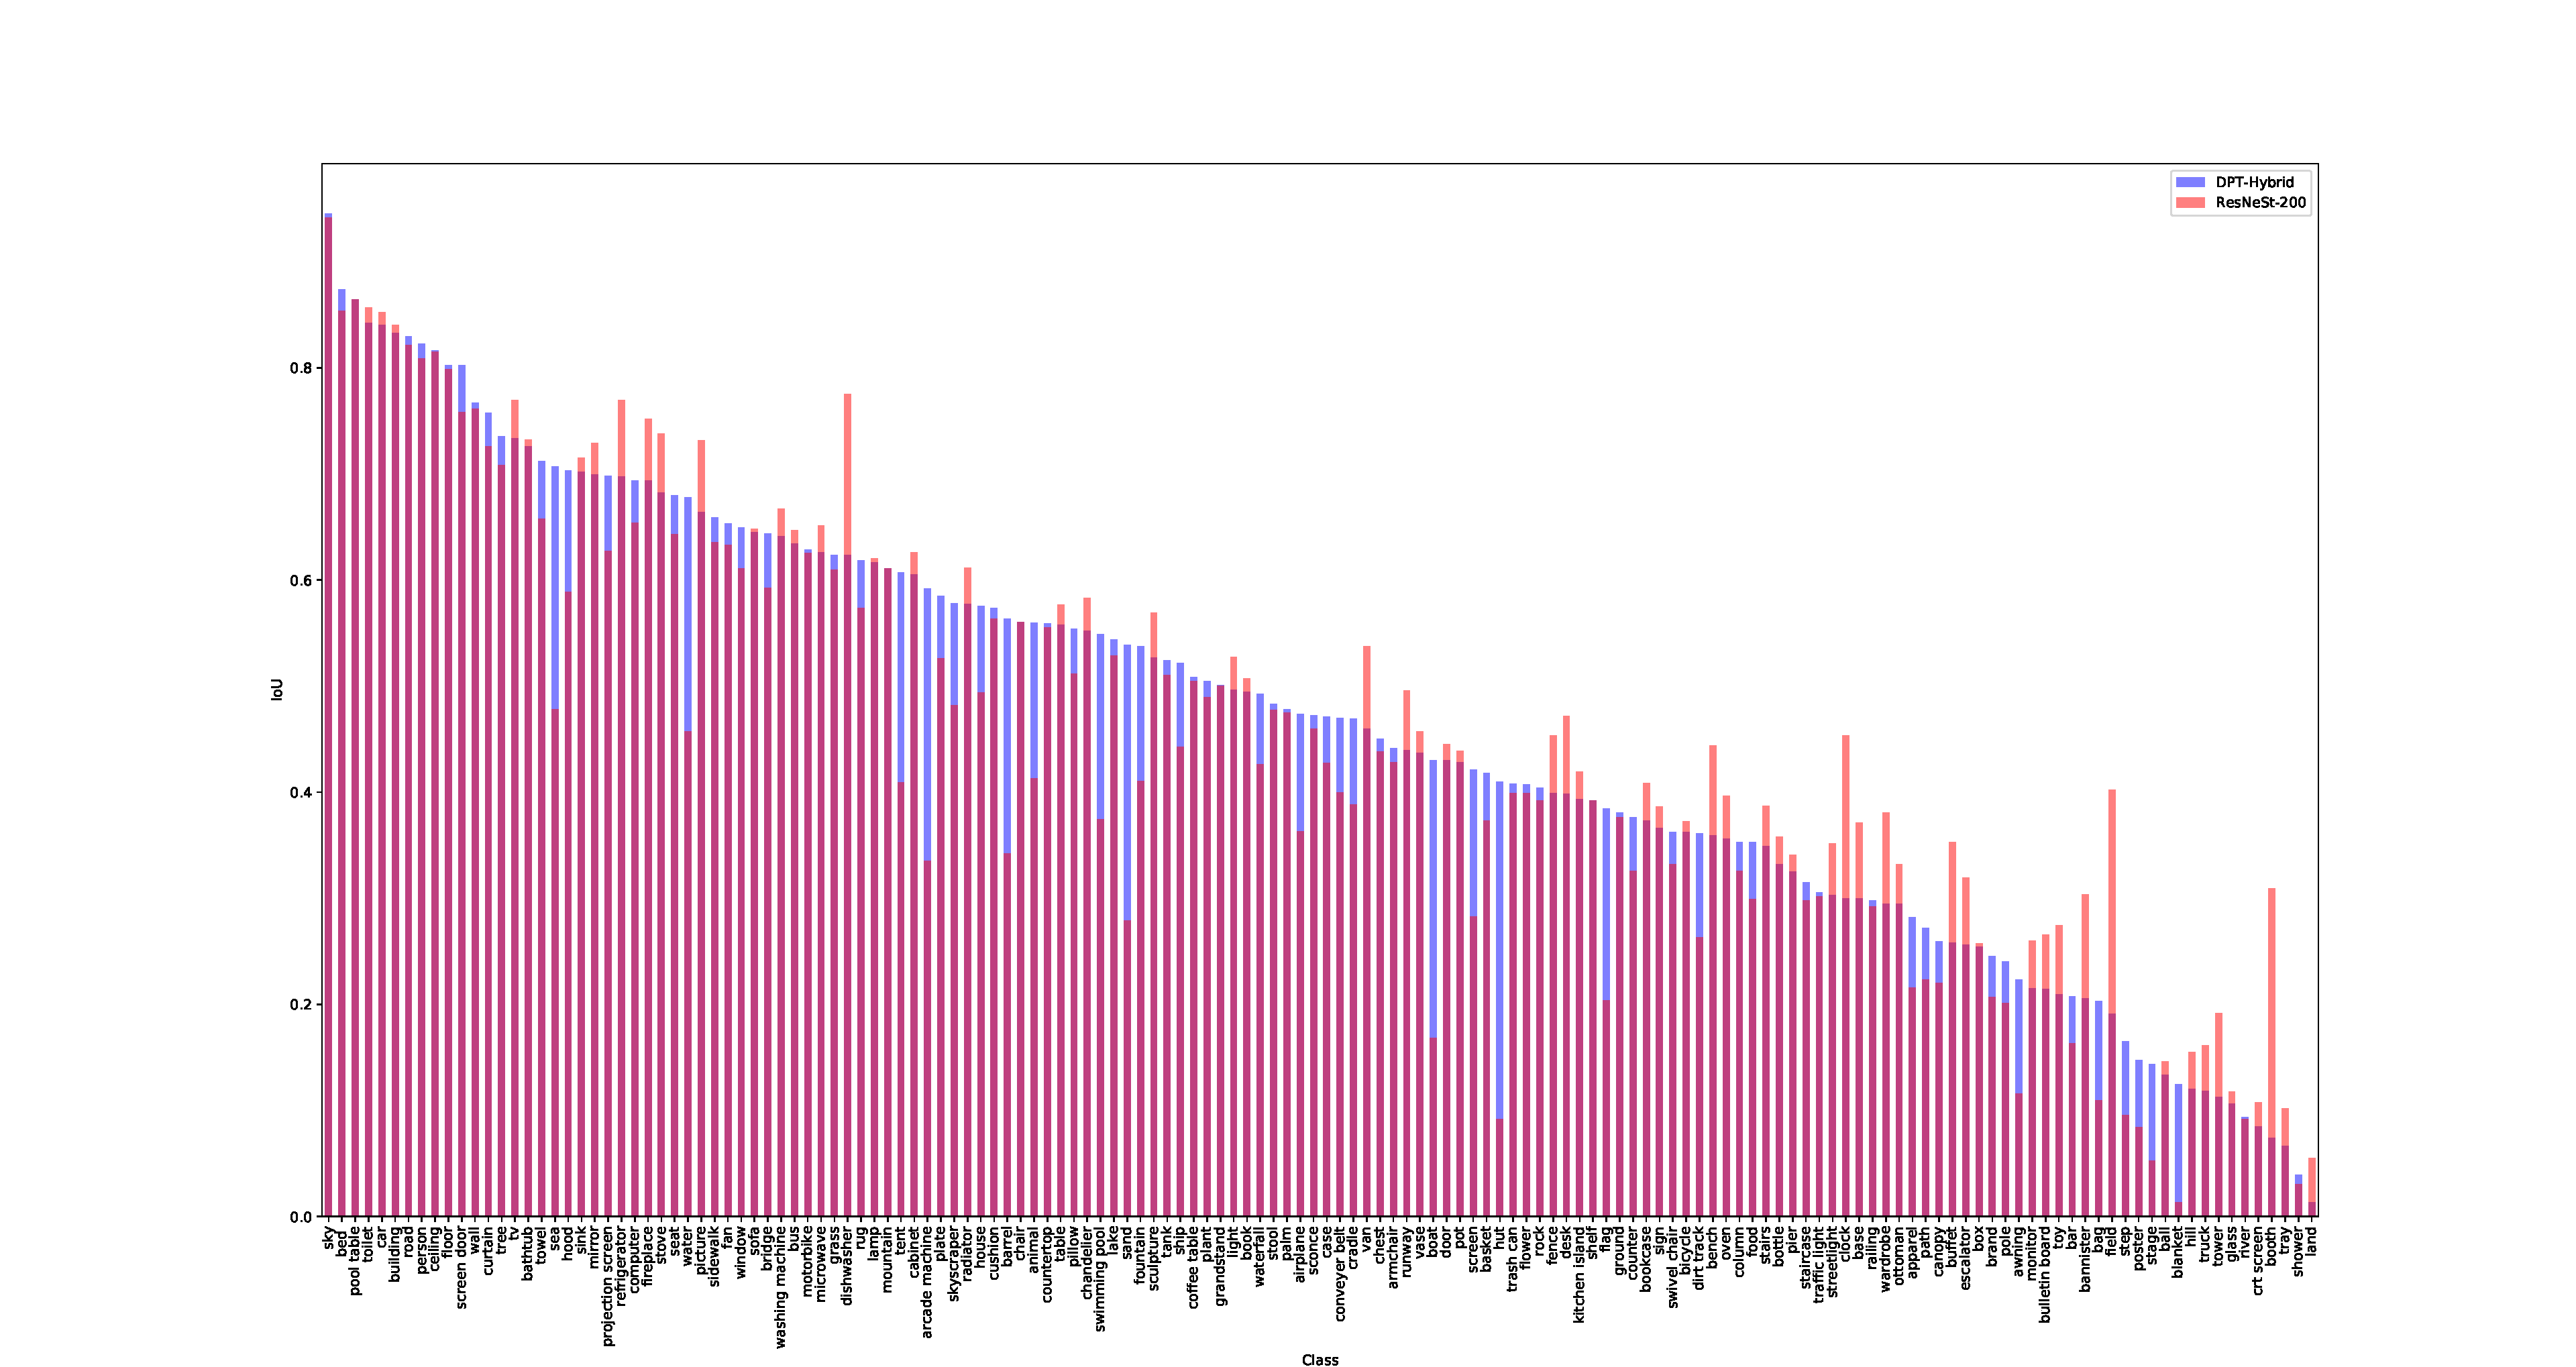
\includegraphics[width=1\linewidth,trim=6.91cm 0 6.51cm 4cm,clip]{images/other/class_iou}
    }
    \caption{Per class IoU on ADE20K.}
  \label{fig:classiou}
\end{figure*}


\mypara{Hybrid encoder.} The hybrid encoder is based on a pre-activation
ResNet50 with group norm and weight standardization \citeappendix{Kolesnikov2020}. It
defines four stages after the initial stem, each of which downsamples the
representation before applying multiple ResNet blocks. We refer by $RN$ to the
output of the $N$-th stage. DPT-Hybrid thus taps skip connections after the
first ($R0$) and second stage ($R1$).

\mypara{Residual convolutional units.}
Figure \ref{fig:archdetails}~(a) shows a schematic overview of the residual convolutional
units \citeappendix{Lin2017} that are used in the decoder. Batch normalization is used for
semantic segmentation but is disabled for monocular depth estimation. When using batch
normalization, we disable biases in the preceding convolutional layer.

\mypara{Monocular depth estimation head.} The output head for monocular depth
estimation is shown in Figure \ref{fig:archdetails}~(b). The initial convolution
halves the feature dimensions, while the second convolution has an output
dimension of $32$. The final linear layer projects this representation to a
non-negative scalar that represent the inverse depth prediction for every pixel.
Bilinear interpolation is used to upsample the representation.


\mypara{Semantic segmentation head.} The output head for semantic segmentation is
shown in Figure \ref{fig:archdetails}~(c). the first convolutional block
preserves the feature dimension, while the final linear layer projects the
representation to the number of output classes. Dropout is used with a rate of
$0.1$. We use bilinear interpolation for the final upsampling operation. The
prediction thus represents the per-pixel logits of the classes.


\section{Additional results}
We provide additional qualitative and quantitative results in this section.

\mypara{Monocular depth estimation.} We notice that the biggest gains in
performance for zero-shot transfer were achieved for datasets that feature
dense, high-resolution evaluations~\citeappendix{Butler2012,Geiger2012,Schoeps2017}.
This could be explained by more fine-grained predictions. Visual inspection of
sample results (\cf Figure~\ref{fig:monodepth_results_supp}) from these datasets
confirms this intuition. We observe more details and also better global depth arrangement
in DPT predictions when compared to the fully-convolutional baseline.  Note that
results for DPT and MiDaS are computed at the same input resolution (384 pixels).

\begin{figure*}[!t]
  \centering
  \def\mywidth{0.32}
  \begin{tabular}{@{}c@{\hspace{1mm}}c@{\hspace{1mm}}c@{}}
    Input & MiDaS (MIX 5) & DPT-Large\\
    \adjincludegraphics[width=\mywidth\linewidth,trim={0 0 0 0},clip]{images/monodepth/supplement/input/frame_0016} &
    \adjincludegraphics[width=\mywidth\linewidth,trim={0 0 0 0},clip]{images/monodepth/supplement/midas_21/frame_0016} &
    \adjincludegraphics[width=\mywidth\linewidth,trim={0 0 0 0},clip]{images/monodepth/supplement/dpt_large/frame_0016}\\
    \adjincludegraphics[width=\mywidth\linewidth,trim={0 0 0 0},clip]{images/monodepth/supplement/input/frame_0013} &
    \adjincludegraphics[width=\mywidth\linewidth,trim={0 0 0 0},clip]{images/monodepth/supplement/midas_21/frame_0013} &
    \adjincludegraphics[width=\mywidth\linewidth,trim={0 0 0 0},clip]{images/monodepth/supplement/dpt_large/frame_0013}\\
    \adjincludegraphics[width=\mywidth\linewidth,trim={0 0 0 0},clip]{images/monodepth/supplement/input/2011_09_26_drive_0002_sync_image_0000000006_image_02} &
    \adjincludegraphics[width=\mywidth\linewidth,trim={0 0 0 0},clip]{images/monodepth/supplement/midas_21/2011_09_26_drive_0002_sync_image_0000000006_image_02} &                                                                                                                                                                          \adjincludegraphics[width=\mywidth\linewidth,trim={0 0 0 0},clip]{images/monodepth/supplement/dpt_large/2011_09_26_drive_0002_sync_image_0000000006_image_02}\\
    \adjincludegraphics[width=\mywidth\linewidth,trim={0 0 0 0},clip]{images/monodepth/supplement/input/2011_09_26_drive_0013_sync_image_0000000100_image_02} &
    \adjincludegraphics[width=\mywidth\linewidth,trim={0 0 0 0},clip]{images/monodepth/supplement/midas_21/2011_09_26_drive_0013_sync_image_0000000100_image_02} &                                                                                                                                                                          \adjincludegraphics[width=\mywidth\linewidth,trim={0 0 0 0},clip]{images/monodepth/supplement/dpt_large/2011_09_26_drive_0013_sync_image_0000000100_image_02}\\

    \adjincludegraphics[width=\mywidth\linewidth,trim={0 0 0 0},clip]{images/monodepth/supplement/input/2011_09_26_drive_0013_sync_image_0000000115_image_02} &
    \adjincludegraphics[width=\mywidth\linewidth,trim={0 0 0 0},clip]{images/monodepth/supplement/midas_21/2011_09_26_drive_0013_sync_image_0000000115_image_02} &
    \adjincludegraphics[width=\mywidth\linewidth,trim={0 0 0 0},clip]{images/monodepth/supplement/dpt_large/2011_09_26_drive_0013_sync_image_0000000115_image_02}\\
    \adjincludegraphics[width=\mywidth\linewidth,trim={0 0 0 0},clip]{images/monodepth/supplement/input/DSC_0322} &
    \adjincludegraphics[width=\mywidth\linewidth,trim={0 0 0 0},clip]{images/monodepth/supplement/midas_21/DSC_0322} &
    \adjincludegraphics[width=\mywidth\linewidth,trim={0 0 0 0},clip]{images/monodepth/supplement/dpt_large/DSC_0322}\\
    \adjincludegraphics[width=\mywidth\linewidth,trim={0 0 0 0},clip]{images/monodepth/supplement/input/DSC_0686} &
    \adjincludegraphics[width=\mywidth\linewidth,trim={0 0 0 0},clip]{images/monodepth/supplement/midas_21/DSC_0686} &
    \adjincludegraphics[width=\mywidth\linewidth,trim={0 0 0 0},clip]{images/monodepth/supplement/dpt_large/DSC_0686}
  \end{tabular}
  \caption{Additional comparisons for monocular depth estimation.}
  \label{fig:monodepth_results_supp}
\end{figure*}

\mypara{Semantic segmentation.} We show per-class IoU scores for the ADE20K
validation set in Figure~\ref{fig:classiou}. While we observe a general trend of
an improvement in per-class IoU in comparison to the baseline \cite{Zhang2020},
we do not observe a strong pattern across classes.

\mypara{Attention maps.} We show attention maps from different encoder layers in
Figures~\ref{fig:attention_large} and~\ref{fig:attention_hybrid}. In both cases, we show
results from the monocular depth estimation models. We visualize
the attention of two reference tokens (upper left corner and lower right corner,
respectively) to all other tokens in the image across various layers in the
encoder. We show the average attention over all $12$ attention heads.

We observe the tendency that attention is spatially more localized close to the
reference token in shallow layers (leftmost columns), whereas deeper layers
(rightmost columns) frequently attend across the whole image.


\begin{figure*}[!t]
  \centering
  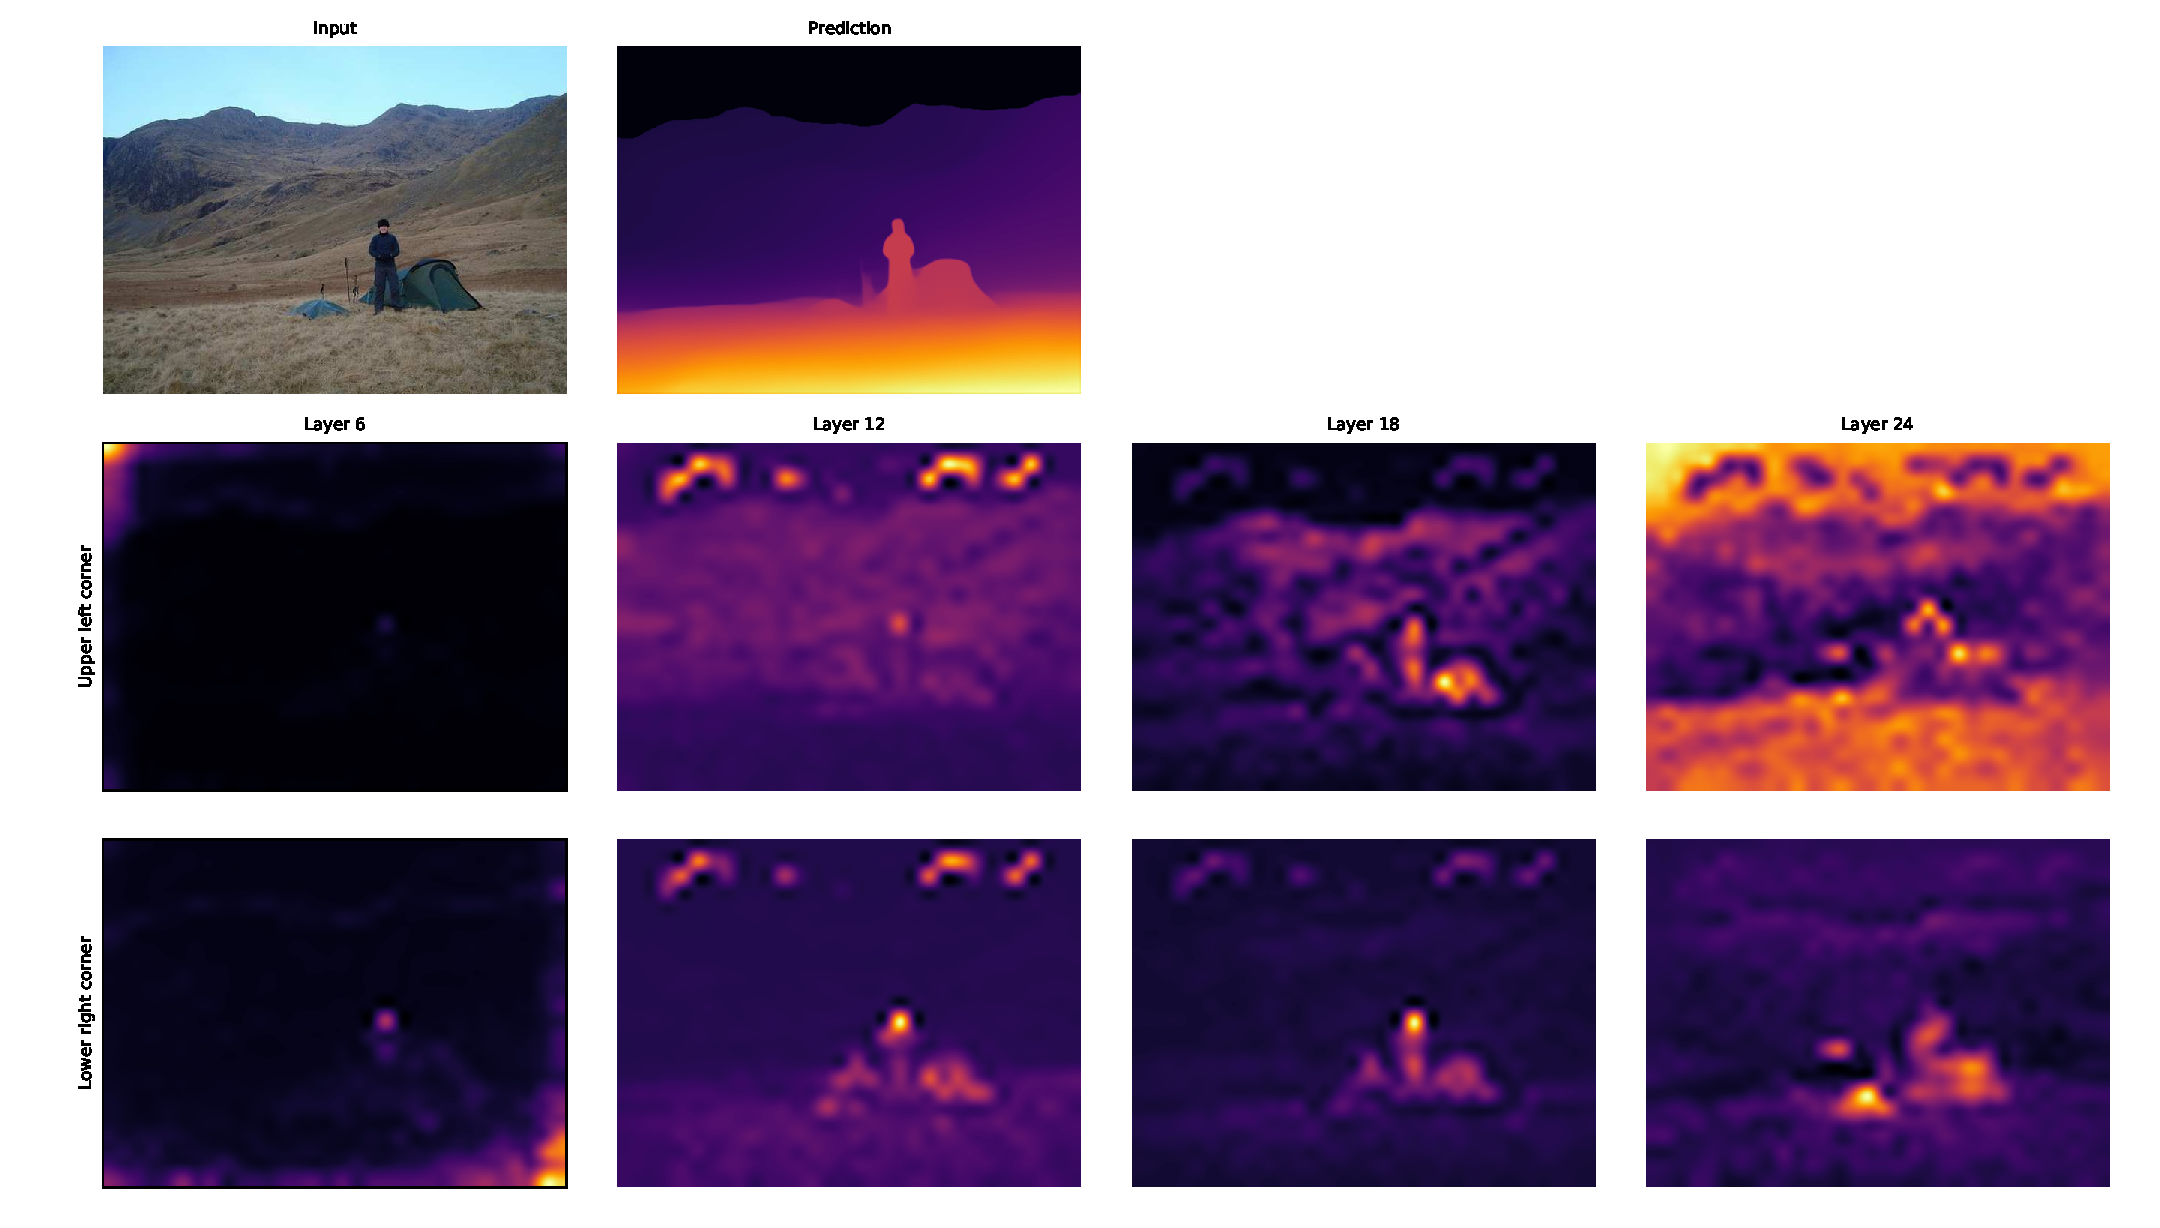
\includegraphics[width=1\textwidth]{images/attention_maps_large/wanderer}\\
  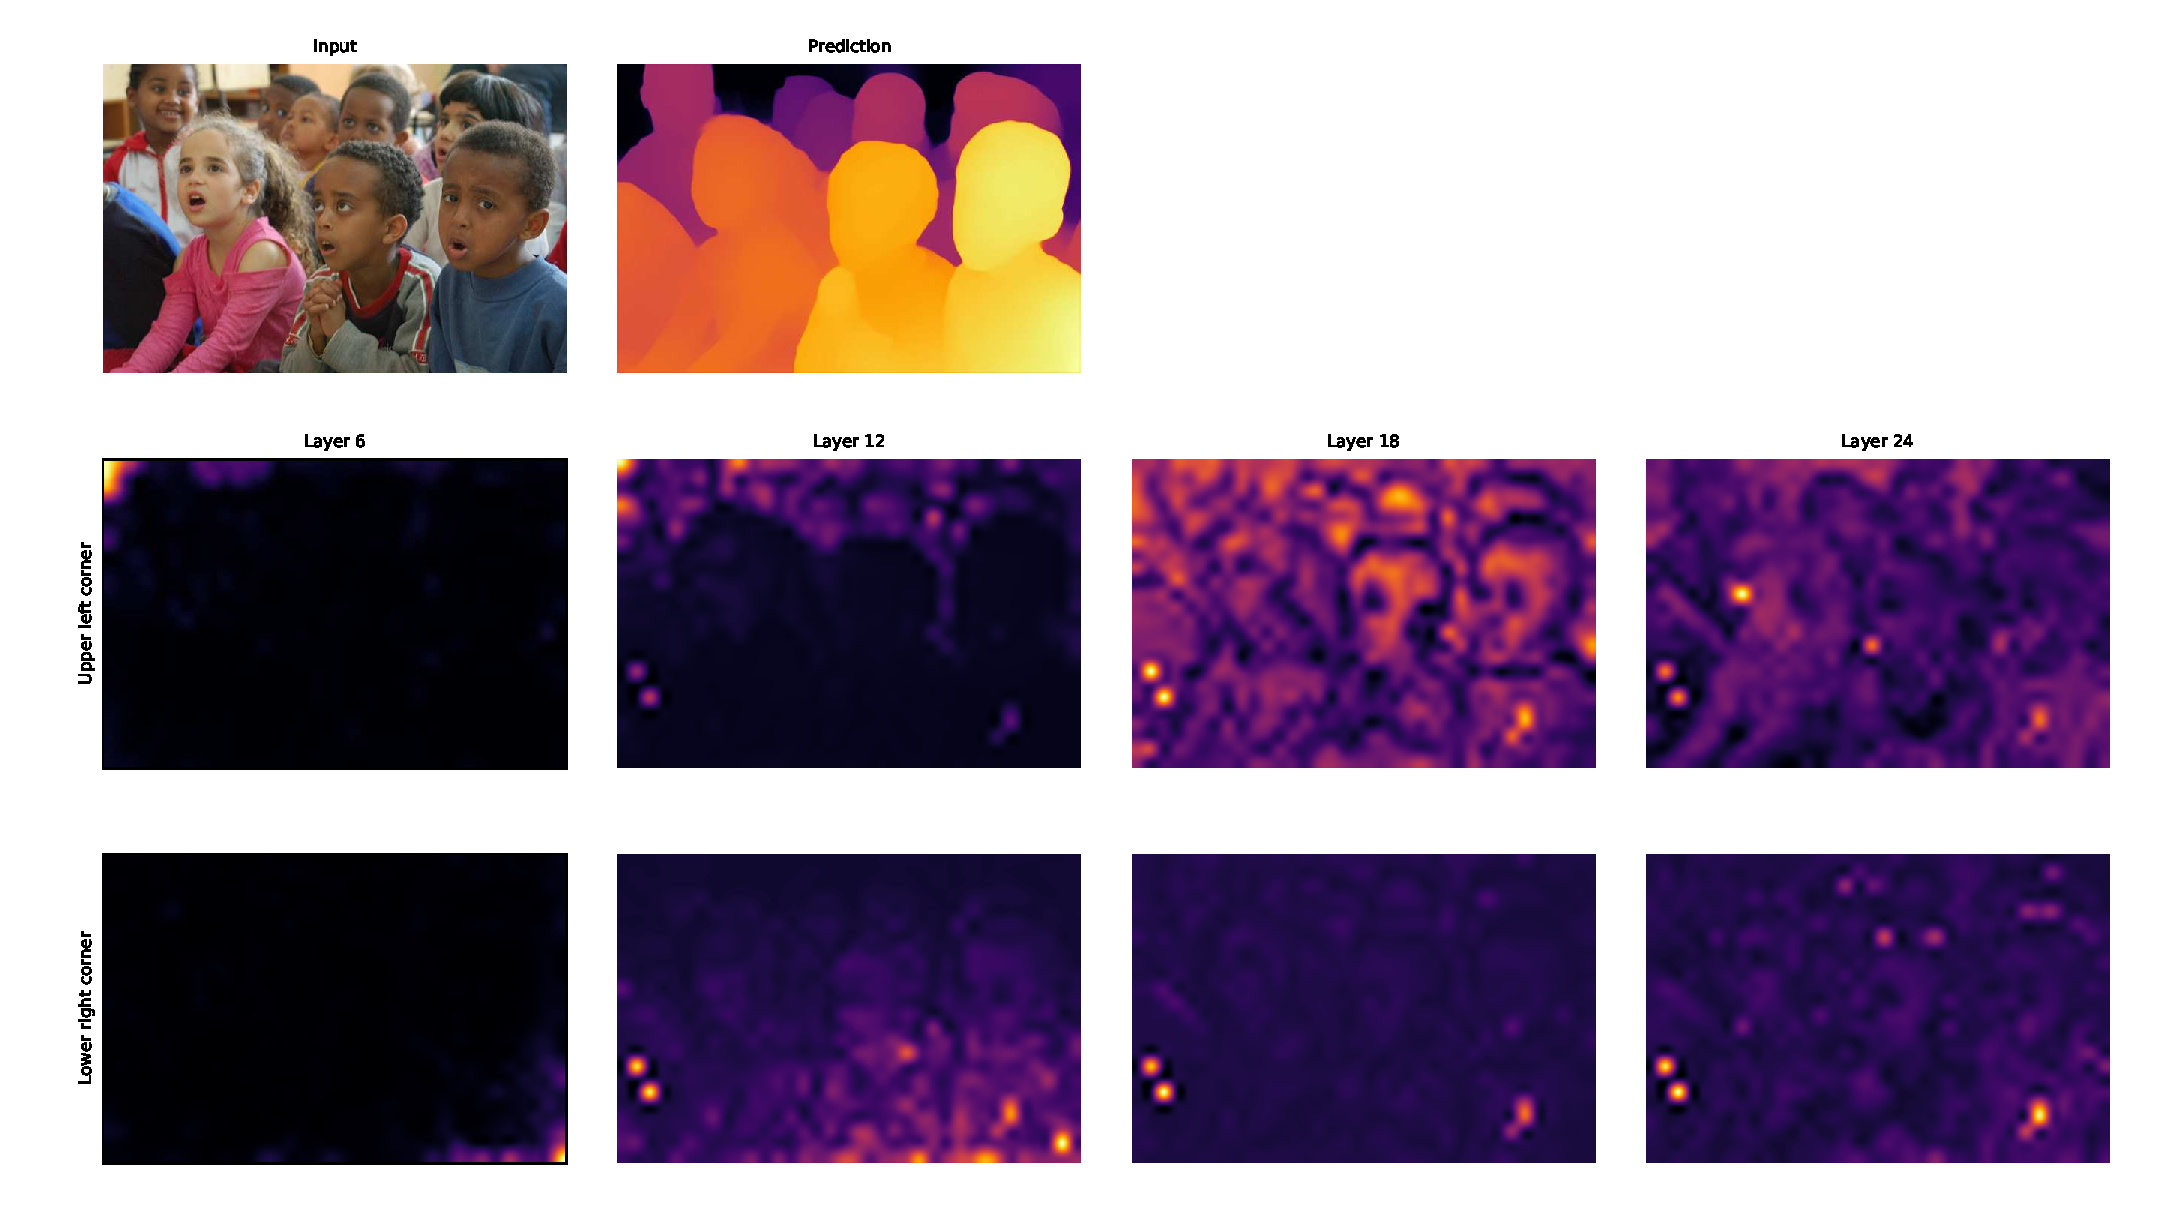
\includegraphics[width=1\textwidth]{images/attention_maps_large/children}
  \caption{Sample attention maps of the DPT-Large monocular depth prediction network.}
  \label{fig:attention_large}
\end{figure*}


\begin{figure*}[!t]
  \centering
  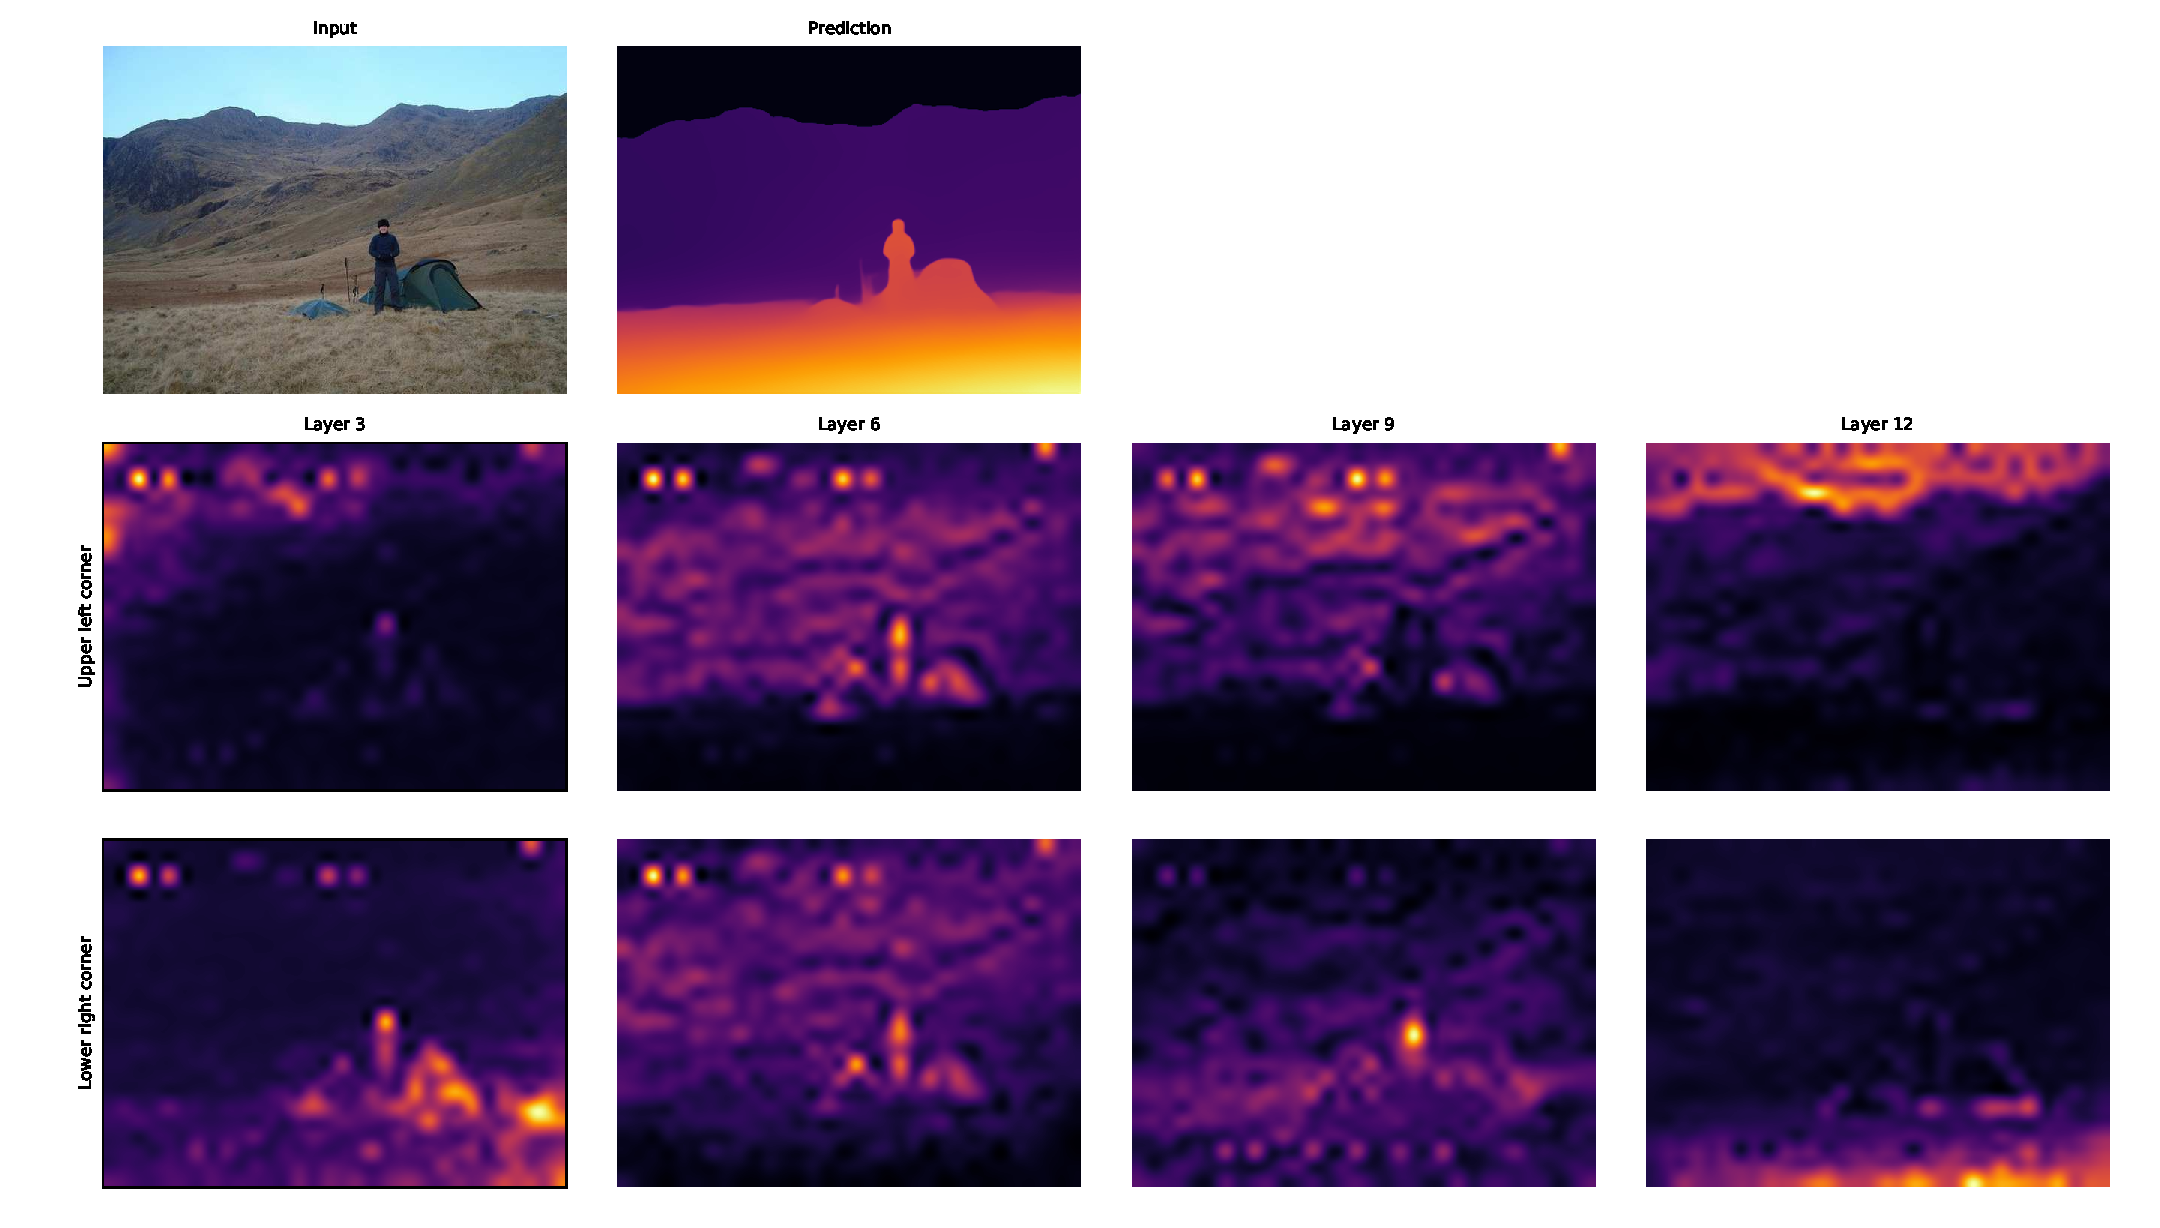
\includegraphics[width=1\textwidth]{images/attention_maps_hybrid/wanderer}\\
  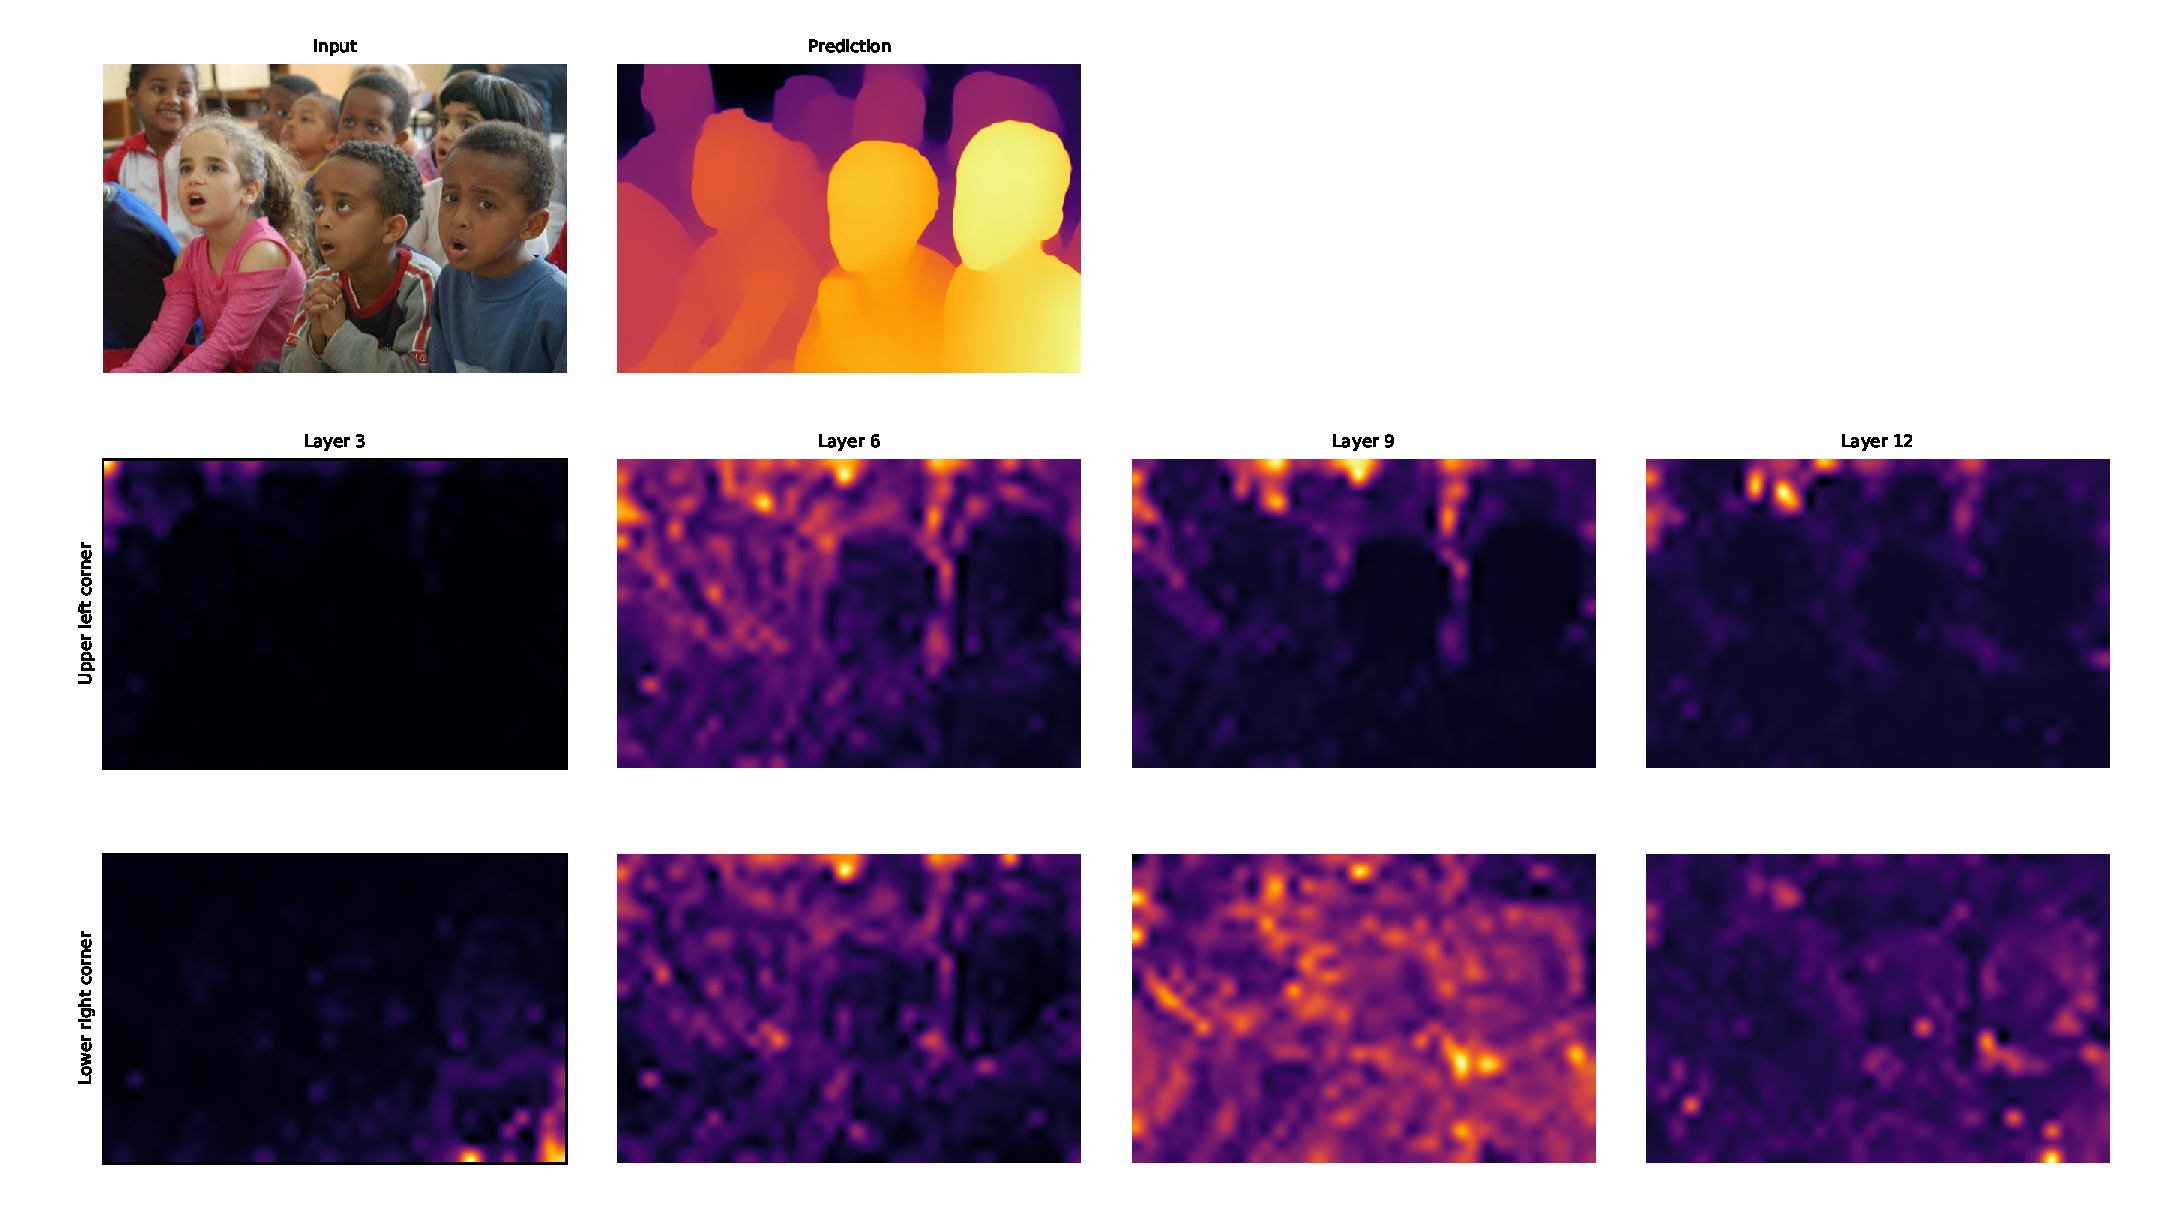
\includegraphics[width=1\textwidth]{images/attention_maps_hybrid/children}
  \caption{Sample attention maps of the DPT-Hybrid monocular depth prediction network.}
  \label{fig:attention_hybrid}
\end{figure*}

{\small \bibliographystyleappendix{ieee_fullname} \bibliographyappendix{egbib}


\end{document}
